\documentclass[upright, contnum]{umemoria}
\deptoA{DEPARTAMENTO DE INGENIERÍA ELÉCTRICA}
\deptoB{DEPARTAMENTO DE CIENCIAS DE LA COMPUTACIÓN}
\author{Matías Fernando Pavez Bahamondes}
\title{Diseño e Implementación de Memoria de Largo Plazo para Robots de Servicio}
\auspicio{}
\date{2018}
\guia{Javier Ruiz del Solar, JOCELYN SIMMONDS WAGEMANN}
\carreraA{INGENIERO CIVIL ELÉCTRICO E}
\carreraB{INGENIERO CIVIL EN COMPUTACIÓN}
\memoria{MEMORIA PARA OPTAR AL TÍTULO DE INGENIERO CIVIL ELÉCTRICO E INGENIERO CIVIL EN COMPUTACIÓN}
\comision{Luis Mateu Brulé, Andrés Caba Rutte}

\usepackage[T1]{fontenc}
\usepackage[spanish]{babelbib}
\usepackage{enumitem} % opciones para itemize 

% ------------- Imágenes -------------------------------------- %
\usepackage[pdftex]{graphicx}	% Para Archivos gráficos         %
\usepackage{float}				% Para usar H!                   %
\usepackage[section]{placeins}	% auto \FloatBarrier por sección %
\usepackage{caption}			% [font=small,labelfont=bf]      %
\usepackage{subcaption}         % Caption para subfiguras        %
\usepackage{sidecap}            % Captions al lado               %
\usepackage{wrapfig}            % Escribir alrededor             %
\graphicspath{{./figures/}}     % Agrega Path para buscar imgs.  %
% ------------------------------------------------------------- %

% = = = = = = = = = = = = = = = = = = = = = = =
% TODO NOTES
% = = = = = = = = = = = = = = = = = = = = = = =
\usepackage[pdftex,dvipsnames,table]{xcolor}  % Coloured text etc.
%\usepackage[colorinlistoftodos,prependcaption,textsize=small]{todonotes}
\usepackage[colorinlistoftodos,prependcaption,textsize=tiny,disable]{todonotes}
\newcommand{\todoimplementation}[1]{\todo[linecolor=blue,backgroundcolor=blue!25,bordercolor=blue,inline]{CODE ME: #1}}
\newcommand{\todopaused}[1]{\todo[linecolor=red,backgroundcolor=red!25,bordercolor=red,inline]{PAUSED: #1}}
\newcommand{\todounsure}[1]{\todo[linecolor=green,backgroundcolor=green!25,bordercolor=green,inline]{UNSURE: #1}}
\newcommand{\todojocelyn}[1]{\todo[linecolor=black,backgroundcolor=cyan!25,bordercolor=blue,inline]{CORRECCIÓN J.Simmonds: #1}}
\newcommand{\todolater}[1]{\todo[linecolor=black,backgroundcolor=black!25,bordercolor=black,inline]{LATER: #1}}
\newcommand{\todofinal}[1]{\todo[linecolor=black,backgroundcolor=black!10,bordercolor=black,inline]{VERSION FINAL: #1}}
\newcommand{\todoimprove}[1]{\todo[linecolor=yellow,backgroundcolor=yellow!25,bordercolor=yellow,inline]{IMPROVEMENT: #1}}
\newcommand{\todowrite}[1]{\todo[linecolor=purple,backgroundcolor=purple!25,bordercolor=purple,inline]{WRITE ME: #1}}
\setlength{\marginparwidth}{0.5in} % mostrar correctamente todos al margen 
% = = = = = = = = = = = = = = = = = = = = = = =


\hypersetup{
	colorlinks,
	linkcolor={black},
	citecolor={blue!50!black},
	urlcolor={blue!80!black}
}

\usepackage{tikz}


%% Sections formatting
% -----------------------------------------

\usepackage{titlesec}
\usepackage[toc]{appendix}
\usepackage{etoolbox}
\makeatletter
% appendix and hyperref packages are broken with utf8!
% https://tex.stackexchange.com/questions/58848/ap%c3%a9ndices-appendix-spanish-accent
\appto{\appendices}{\def\Hy@chapapp{Appendix}}

% title sec is bugged on texlive-full deb. use this to correct it.
% Source: https://bugs.launchpad.net/ubuntu/+source/texlive-extra/+bug/1574052
\patchcmd{\ttlh@hang}{\parindent\z@}{\parindent\z@\leavevmode}{}{}
\patchcmd{\ttlh@hang}{\noindent}{}{}{}
\makeatother
% -----------------------------------------
% less spaced \paragraph sections
\titlespacing{\paragraph}{0pc}{0.0ex plus .1ex minus .2ex}{1pc}
%{12pc}{1.5ex plus .1ex minus .2ex}{1pc}

% Fancy chapters.. more on: https://ctan.org/pkg/fncychap
%Options: Sonny, Lenny, Glenn, Conny, Rejne, Bjarne, Bjornstrup, PetersLenny
\usepackage[Bjornstrup]{fncychap}

% Numbering and TOC for: 
% Chapters(0), Sections(1), subsections(2), subsubsections(3)
\setcounter{tocdepth}{2}
\setcounter{secnumdepth}{3}

% highlight
\usepackage{soul}
%\setulcolor{red}
%\sethlcolor{blue}
%\renewcommand\ul[1]{#1} % <<<<<<<<<<<<<<<<<<<<<<<<<<<<<<<<<<<<<
%\renewcommand\hl[1]{#1} % <<<<<<<<<<<<<<<<<<<<<<<<<<<<<<<<<<<<<


%%----- Colores --------------------------------------------------%
%\usepackage{color}												%
%\usepackage{colortbl}											%
%\usepackage[usenames,dvipsnames,svgnames,table]{xcolor}			%
%\definecolor{gray}{rgb}{0.51,0.51,0.51}							%
%\definecolor{dkgreen}{rgb}{0,0.6,0}								%
%\definecolor{mauve}{rgb}{0.58,0,0.82}							%
%%----------------------------------------------------------------%


% -------------------------------------------------------------------- %
% ----- LISTINGS ----------------------------------------------------- %
% -------------------------------------------------------------------- %
\usepackage{listingsutf8}

\renewcommand{\lstlistingname}{C\'odigo}
\renewcommand{\lstlistlistingname}{Listado de \lstlistingname s}

% --------------------------------------------------------%
% --------------- ESTILOS  -------------------------------%
% --------------------------------------------------------%
\lstdefinestyle{/Style/code}{
	%
	% ---- structure ----
	%title=\lstname,                    % show filename of files of title
	caption=\lstname,                   % also try caption instead
	captionpos=t,                       % caption-position to bottom
	basicstyle=\scriptsize\ttfamily,    % \footnotesize
	columns=fullflexible,               % %fixed
	tabsize=2,
	aboveskip={1.5\baselineskip},
	%
	% ---- numbers ----
	numbers=left,
	stepnumber=1,
	numbersep=5pt,                      % distance(line-numbers, code)
	numberstyle=\tiny\color{gray},      % for line-numbers	
	%
	% ---- shows ----
	showspaces=false,                   % spaces with particular underscores
	showstringspaces=false,             % underline spaces within strings
	showtabs=false,                     % tabs with particular underscores
	frame=false,                        % adds a frame around the code 
	%                                   % false, tb, shadowbox, single, lines
	%
	% ---- color ----
	backgroundcolor=\color{white},
	rulecolor=\color{black},
	%
	% ---- break ----
	breakatwhitespace=false,            % automatic breaks should only happen at whitespace
	breaklines=true,                    % automatic line breaking
	%                                   % Simbolo mostrado para el breakline
	prebreak = \raisebox{0ex}[0ex][0ex]{\ensuremath{\hookleftarrow}},
	%
	% ---- Extras ----
	%escapeinside={\%*}{*)},         	% LaTeX within your code
	extendedchars=true,
	inputencoding=utf8/latin1 			% Tildes
}

\lstdefinestyle{/Style/C}{
	language=C,
	keywordstyle=\bfseries\ttfamily\color[rgb]{0,0,1},
	identifierstyle=\ttfamily,
	commentstyle=\color[rgb]{0.133,0.545,0.133},
	stringstyle=\ttfamily\color[rgb]{0.627,0.126,0.941},
	style=/Style/code
}
\lstdefinestyle{/Style/C++}{
	language=C++,
	keywordstyle=\bfseries\ttfamily\color[rgb]{0,0,1},
	identifierstyle=\ttfamily,
	commentstyle=\color[rgb]{0.133,0.545,0.133},
	stringstyle=\ttfamily\color[rgb]{0.627,0.126,0.941},
	style=/Style/code
}

% --- XML de ROS ----------->
\lstdefinelanguage{/XML/ROS}{
	sensitive=false,
	morestring=[b]",
	%morestring=[s]{>}{<},
	morecomment=[s]{<!--}{-->},
	morecomment=[s]{<?}{?>},
	morekeywords={master, include, launch, node, param, rosparam, group, machine, arg} % list of attributes
}

\lstdefinestyle{/Style/XML/ROS}{
	language=/XML/ROS,
	stringstyle=\color{WildStrawberry},
	identifierstyle=\color{RoyalPurple},
	keywordstyle=\color{Emerald},
	%commentstyle=\color{Purple},	de los <? ?>
	commentstyle=\color{Blue},
	style=/Style/code
}
\lstdefinestyle{/Style/sh}{
	language=sh,
	stringstyle=\color{WildStrawberry},
	identifierstyle=\color{RoyalPurple},
	keywordstyle=\color{red},
	commentstyle=\color{Blue},
	style=/Style/code
}


% --- YAML de ROS ----------->
\newcommand\YAMLcolonstyle{\color{red}\mdseries}
\newcommand\YAMLkeystyle{\color{black}\bfseries}
\newcommand\YAMLvaluestyle{\color{blue}\mdseries}
\lstdefinelanguage{/YAML/ROS}{
    sensitive=false,
    morestring=[b]",
    morestring=[b]',
    moredelim=**[il][\YAMLcolonstyle{:}\YAMLvaluestyle]{:},
    morecomment=[l]{\#}
}
\lstdefinestyle{/Style/yaml/ROS}{
	language=/YAML/ROS,
	stringstyle=\color{Green},
	identifierstyle=\color{Black},
	keywordstyle=\color{Red},
	commentstyle=\color{Gray},
	style=/Style/code
}


% colores disponibles: https://en.wikibooks.org/wiki/LaTeX/Colors
% --- MSG de ROS ----------->
\lstdefinelanguage{/ROS/MSG}{
	%	alsodigit={-},
	alsoletter={},
	sensitive=true,
	comment=[l]{\#},
	keywords=[1]{
		uint32, uint8, string, float32, int32, bool, time,
		geometry\_msgs,Point,sensor\_msgs,Image
	},
	keywords=[2]{
		ltm, ltm\_samples, What, When, Where, Episode,
		Info, Date, Relevance, EmotionalRelevance, HistoricalRelevance
	},
	%otherkeywords={---,=}
}
\lstdefinestyle{/Style/ROS/MSG}{
	language=/ROS/MSG,
	stringstyle=\color{Green},
	identifierstyle=\color{Black},
	keywordstyle=[1]\bf\color{Red},
	keywordstyle=[2]\bf\color{Blue},
	commentstyle=\color{Gray},
	style=/Style/code
}

% --- JSON SAMPLE ----------->
\lstdefinelanguage{/MEM/JSON}{
	%	alsodigit={-},
	alsoletter={},
	sensitive=true,
	comment=[l]{\#},
	string=[s]{"}{"},
	keywords={\$in, \$or, \$gt},
}
\lstdefinestyle{/Style/JSON}{
	language=/MEM/JSON,
	stringstyle=\color{blue},
	identifierstyle=\color{Black},
	keywordstyle=\bf\color{Red},
	commentstyle=\color{Gray},
}


% custom caption for listings
\usepackage{caption}
\DeclareCaptionFont{listingfont}{\color{white}}
\DeclareCaptionFont{listinglabelfont}{\bf\color{white}}
\DeclareCaptionFormat{listing}{\colorbox{gray}{\parbox{\textwidth}{#1#2#3}}}
\captionsetup[lstlisting]{format=listing,labelfont=listinglabelfont,textfont=listingfont}


\renewcommand\appendixtocname{Anexos}


% Fuentes para requesitos y validaciones
\newcommand{\RPlabel}[1]{$\mathcal{RP}_{#1}$}
\newcommand{\RStachowicz}[1]{($\mathcal{R}_{#1}$)}
%\newcommand{\RSlabel}[1]{{\bfseries RS{#1}}}
\newcommand{\RSlabel}[1]{{RS{#1}}}
\newcommand{\RPlabelDef}[1]{(\RPlabel{#1}):}
%\newcommand{\Vlabel}[2]{{\bfseries V{#1}{#2}}}
\newcommand{\Vlabel}[2]{{V{#1}{#2}}}
\newcommand{\ltmconcept}[1]{\noindent{\bfseries #1:}\hspace{1em}}

\usepackage{xcolor}
\usepackage{soul}
\definecolor{Light}{gray}{.90}
\sethlcolor{Light}
\let\OldTexttt\texttt
\renewcommand{\texttt}[1]{\OldTexttt{\hl{#1}}}

\newcommand{\CC}{C\nolinebreak\hspace{-.05em}\raisebox{.4ex}{\tiny\bf +}\nolinebreak\hspace{-.10em}\raisebox{.4ex}{\tiny\bf +}}
\def\CC{{C\nolinebreak[4]\hspace{-.05em}\raisebox{.4ex}{\tiny\bf ++}}}


\addto\captionsspanish{%
	\renewcommand{\listfigurename}{Índice de Figuras}
}

\begin{document}

\frontmatter
\maketitle

\begin{abstract}
	\todolater{Abstract.}
\end{abstract}

%\begin{dedicatoria}
\todofinal{Escribir una dedicatoria corta.}
\end{dedicatoria}

\begin{thanks}
\todofinal{Escribir agradecimientos.}

% PÁRRAFOS
% - Conductor de bus que me atropelló... para tener más tiempo para trabajar en la memoria
% - Familia
% - Amigos .. partidas de hots... webeo diario para que trabaje en la cuestion
% - Homebreakers
% - Profesora Jocelyn Simmonds por sus correcciones y consejos.
% - ... JR por darme más y más pega, sin proveer consejos útiles.

\end{thanks}


\cleardoublepage
\tableofcontents
%\cleardoublepage
%\listoftables
\cleardoublepage
\listoffigures
%\cleardoublepage
%\lstlistoflistings

\listoftodos

\mainmatter

\chapter{Introducción}\label{chapter:introduction}

\todo{INTRO: MIGRAR DESDE PREINFORME}
\todo[inline]{Intro: Descripción del capítulo}

\section{Antecedentes Generales}

\todo[inline]{Intro: Descripción de antecedentes}

\subsection{Robots de servicio domésticos}
% - 
% - 
% - 

\subsection{Equipo de trabajo: UChile Homebreakers}
% - 
% - 
% - 

\subsection{La memoria humana}
% - 
% - 
% - 


\section{Motivación}

\todo[inline]{Intro: Importancia de la memoria a largo plazo}

\subsection{Problema}
% - Implementación anterior de memoria a largo plazo
%    - No integrada correctamente
%    - Muy limitada
%    - Requiere de mucha intervención del equipo!. No mantenida
% - No existen software alternativos para resolver este problema.

\subsection{Oportunidad}
% - Diseño basado en requerimientos episódicos (cumplirlos todos)
% - Servidor genérico que no fuerce implementaciones y no limitado a sólo 1 robot
% - Arquitectura no invasiva y mantenible
% - Capacidad de integración a futuro en módulos de inferencia


\section{Objetivos del Proyecto}

\subsection{Objetivo general}
% - 
% - 
% - 

\subsection{Objetivos específicos}
% - 
% - 
% - 

\subsection{Alcances y contribución del trabajo}
% - 
% - 
% - 


\section{Estructura de la Memoria}
% - 
% - 
% - 
\todofinal{Agregar summary al final de cada cap.}
\chapter{Marco Teórico}\label{chapter:theory}

En este capítulo se revisan los temas y conceptos relevantes para el desarrollo del trabajo. Se formaliza la definición de robot doméstico y sus alcances. Se describe la memoria humana, sus categorías, funcionamiento y procesos cerebrales relevantes. Basado en los temas anteriores, se revisa la relación entre robótica y la memoria humana: se describen algunos enfoques existentes y las reglas generales para su implementación.


%% =====================================================================
\section{Robots de servicio domésticos}\label{sec:domestic_robots}
%% =====================================================================

La Federación Internacional de Robótica (IFR) \cite{IFR} define \textit{robot} como:
\begin{quotation}
	``Un mecanismo actuado y programable en dos o más ejes y con un cierto grado de autonomía, que se mueve en su entorno para realizar tareas previstas. En este contexto, autonomía se refiere a la habilidad de realizar tareas previstas, basado en el estado actual y lo sensado, sin intervención humana.''
\end{quotation}

Asimismo, la IFR define un \textit{robot de servicio} como un robot ``que realiza tareas útiles para humanos o equipamiento, excluyendo aplicaciones de automatización industrial''. Así, un robot de servicio debe trabajar en ambientes no controlados y con la autonomía suficiente que le permita llevar a cabo su cometido. Generalmente, la robótica de servicio se enfoca en asistir a los seres humanos en tareas repetitivas y comunes.

Según su área de aplicación, un robot de servicio se clasifica en \textit{de uso personal} o \textit{de uso profesional}. Los primeros son utilizados en ambientes no comerciales y por personas comunes; como por ejemplo, un robot sirviente o una silla de ruedas autónoma. Un robot de servicio profesional se utiliza en ambientes comerciales, usualmente operados por alguien entrenado; un ejemplo son los robots de entrega de paquetes o para cirugía.


Según la recopilación de datos realizada por la IFR durante el 2016, este tipo de robots es utilizado en las siguientes áreas:
\begin{itemize}[topsep=0pt]
	\setlength\itemsep{0.2em}
	\item Tareas domésticas: De compañía, asistencia, limpieza, cuidado del hogar.
	\item Entretenimiento: Juguetes, comunicación, educación e investigación.
	\item Asistencia a ancianos y discapacitados: Sillas robóticas y robots para cuidar personas.
	\item Transporte.
	\item Seguridad y vigilancia.
	\item Otros que no caen en las categorías anteriores.
\end{itemize}
\bigskip

El foco de este trabajo son los robots de servicio personales, dedicados a tareas domésticas, clasificación a la que en  adelante se referirá como \textit{Robots Domésticos}.

Para entender el alcance del trabajo, en cuanto a qué es lo que se espera del sistema, a continuación se listan algunas capacidades de los robots domésticos. Un robot de compañía y asistencia tiene, pero no se limita a las siguientes tareas:
\begin{itemize}[topsep=0pt]
	\setlength\itemsep{0.2em}
	\item Interacción amistosa con humanos.
	\item Ayudar a recordar y organizar tareas.
	\item Cooperar con la realización de un procedimiento.
	\item Guiar y seguir a personas.
	\item Recordar información y entidades.
\end{itemize}
\bigskip

Algunas tareas que robots domésticos de tipo mayordomo deben ejecutar son:
\begin{itemize}[topsep=0pt]
	\setlength\itemsep{0.2em}
	\item Ofrecer comida y bebestibles.
	\item Preparación de comida.\setcounter{tocdepth}{4}
	\item Ordenar y limpiar el hogar.
\end{itemize}
\bigskip

El primero de los objetivos específicos del proyecto tiene que ver con la derivación de consultas útiles para validar la memoria, a partir de las capacidades esperadas para un robot de servicio doméstico. En el Capítulo \ref{chapter:metodologia} se presenta cómo se planea desarrollar esta tarea.


%% =====================================================================
\section{Memoria humana}\label{sec:human_memory}
%% =====================================================================

\todoimprove{Poner referencias a todo esto. ... psicoanalisis ... ciencias cognitivas.}
% \cite{Deutsch2008} 

La memoria es un elemento fundamental para los humanos en su día a día, es parte integral de su existencia. Permite recordar quién, qué, cómo, dónde y cuándo. En términos psicológicos, es la habilidad para para codificar, almacenar y luego obtener información sobre eventos pasados, en el cerebro. Los pensamientos son parte de la memoria de corto plazo, mientras que eventos pasados son almacenados en una memoria de largo plazo. Existen muchos estudios en el área de la psicología cognitiva con diversas descripciones y modelos teóricos de cada tipo de memoria \cite{Vijayakumar2014}.

Desde el punto de vista de la información procesada, la memoria es vista como una facultad humana consistente en procesos para el manejo de información. Los 3 componentes principales son:

\begin{itemize}[topsep=0pt]
	\setlength\itemsep{0.2em}
	\item Codificación: En este paso, se adquiere nueva información desde los sentidos humanos. Los datos son convertidos a un formato que pueda ser almacenado en la estructura cerebral correspondiente.
	\item Almacenamiento: Consiste en la creación de registros permanentes de información. Es un proceso pasivo, de continuo procesamiento para clasificar datos nuevos y los ya existentes en el cerebro.
	\item Adquisición: Hace referencia al acceso de datos almacenados. El proceso se realiza en el momento, para obtener una reconstrucción aproximada de la información, a partir de elementos repartidos en distintas partes del cerebro.
\end{itemize}
%\bigskip


La memoria puede ser dividida en múltiples sistemas de independientes, con funcionalidades bien definidas y sustentados por distintas estructuras cerebrales. La primera diferenciación define dos tipos de memoria: la memoria de corto y la de largo plazo, STM (Short-Term Memory) y LTM (Long-Term Memory), por sus siglas en inglés. En el diagrama de la Figura \ref{img:human_memory} se muestra una separación clásica utilizada en el área de las ciencias cognitivas \cite{Eichenbaum:2008}, explicada en las siguientes subsecciones.

\usetikzlibrary{arrows,shapes,positioning,shadows,trees}
\tikzset{
	basic/.style  = {draw, drop shadow, font=\sffamily, rectangle},
	root/.style   = {basic, rounded corners=2pt, text width=10em, very thick, align=center, fill=gray!5},
	level 1/.style = {sibling distance=20mm},
	level 2/.style = {basic, rounded corners=6pt, thin,align=center, fill=red!10, text width=8em},
	level 3/.style = {basic, rounded corners=2pt, thin, align=center, fill=gray!10, text width=6.5em},
	level 4/.style = {basic, thin, align=left, fill=blue!10, text width=10em}
}

\begin{figure}[!h]
	\centering
	\begin{tikzpicture}[]
	
	\node [root] {Memoria Humana}
	child { node [level 2, xshift=-70pt] (c1) {\footnotesize Corto Plazo\\ (STM) }}
	child { node [level 2, xshift=100pt] (c2) {\footnotesize Largo Plazo\\ (LTM) }};
	
	\begin{scope}[every node/.style={level 3}]
	\node [below of = c2, xshift=-80pt, yshift=-20pt] (c21) {\footnotesize Explícita\\ (consciente)};  
	\node [below of = c2, xshift=80pt, yshift=-20pt] (c22) {\footnotesize Implícita\\ (inconsciente)};
	\end{scope} 
	
	\begin{scope}[every node/.style={level 4}]
	\node [below of = c21, xshift=40pt, yshift=-10pt] (c211) {\footnotesize Episódica (Ep-LTM)};
	\node [below of = c211, xshift=0pt, yshift=0pt] (c212) {\footnotesize Semántica (S-LTM)};
	
	\node [below of = c22, xshift=40pt, yshift=-10pt] (c221) {\footnotesize Procedural (P-LTM)};
	\node [below of = c221, xshift=0pt, yshift=0pt] (c222) {\footnotesize Primado};
	\node [below of = c222, xshift=0pt, yshift=0pt] (c223) {\footnotesize Emocional (Em-LTM)};
	\end{scope} 
	
	\draw[-, to path={-- (\tikztotarget)}]
	(c2) edge (c21)
	(c2) edge (c22);
	
	\draw[-, to path={|- (\tikztotarget)}]
	(c21.195) edge (c211.west)
	(c21.195) edge (c212.west);
	
	\draw[-, to path={|- (\tikztotarget)}]
	(c22.195) edge (c221.west)
	(c22.195) edge (c222.west)
	(c22.195) edge (c223.west);
	
	%
	
	%\draw[->, to path={-| (\tikztotarget)}]
	%  (c21) edge (c211) (c21) edge (c212);
	
	\end{tikzpicture}
	\caption{\small Clasificaciones de la memoria humana.}
	\label{img:human_memory}
\end{figure}


% Sobre el estudio de la memoria.. origenes.. Tulving 


\subsection{Memoria de corto plazo}
% - 
% - 
% - 
En el ámbito cognitivo, la STM se refiere a la habilidad de estar atento, recopilar información  y memorias, para luego utilizarlas dentro de un corto periodo de tiempo. Es responsable de almacenar información constantemente y de decidir que parte será transferida a la memoria de largo plazo. El término de \textit{Memoria de Trabajo} suele ser utilizado de manera intercambiable con el de STM.

La STM se caracteriza por manejar información muy detallada, ser de poca capacidad y permitir un rápido acceso a estos datos. Permite recordar rápidamente y con gran detalle experiencias ocurridas hace pocos segundos, pero con dificultad creciente a medida que avanza el tiempo.

Se sustenta principalmente en la corteza prefrontal del cerebro. Algunos estudios han mostrado que las neuronas involucradas son capaces de mantener información relevante de corto plazo, la que es combinada con información sensorial entrante y áreas que manejan la toma de decisiones. %(Miller, 2000).
En los humanos esta área presenta gran activación durante procesos de codificación, acceso y manipulación de memorias. %(Postle, 2006). 


\subsection{Memoria de largo plazo}

La LTM se asocia al almacenamiento permanente de información en el cerebro. Se caracteriza por manejar mucha información sobre experiencias y entidades, ser menos detallada y proveer un acceso más lento a los recuerdos, respecto a la STM \cite{Eichenbaum:2008}. Cierta información de la STM eventualmente es transferida a la LTM. De acuerdo a la Figura \ref{img:human_memory}, sus dos principales categorías son la \textit{Memoria Implícita} y la \textit{Memoria Explícita}.
% algunos creen que no está limitada en su capacidad de almacenar información.

\subsubsection{Memoria de largo plazo explícita}

La memoria explícita suele ser denominada \textit{memoria consciente} o \textit{memoria declarativa}, pues maneja conocimientos relacionados a hechos y eventos adquiridos de forma consciente. Según las estructuras cerebrales involucradas, se conforma de la \textit{memoria episódica} y de la \textit{memoria semántica}.

La memoria episódica (Ep-LTM) es de carácter  autobiográfico y almacena detalles de eventos y experiencias pasadas. Permite responder a las preguntas ``Qué sucedió'', ``Dónde ocurrió'' y ``Cuándo ocurrió''. Un humano puede acceder a esta memoria si es capaz de decir: ``recuerdo que''. Este tipo de memoria da al ser humano la sensación de continuidad en el tiempo.

La memoria semántica (S-LTM) almacena el conocimiento de hechos, significados, categorías y proposiciones. Un humano puede acceder a esta memoria si es capaz de decir: ``sé que''. Esta memoria se abstrae de perspectiva e información situacional.

Las estructuras cerebrales que soportan la memoria explícita son el hipocampo, encargado de manejar la Ep-LTM, junto a la corteza cerebral, en donde se distribuyen los conocimientos de la S-LTM. En el hipocampo se mantienen conexiones neuronales a los sectores de interés de la corteza, en donde se alojan conocimientos semánticos asociados a cada episodio.

Un ejemplo de uso de Ep-LTM es el recuerdo de una graduación escolar, el lugar y la fecha donde ocurrió. La S-LTM podría responder en que consiste una graduación y describir la ropa que se suele ocupar en ellas.


\subsubsection{Memoria de largo plazo implícita}

La memoria implícita  abarca la capacidad de aprender habilidades, hábitos y preferencias, caracterizados por ser mejorados o adquiridos sin una recolección consciente. Así, también suele ser denominada \textit{memoria inconsciente} o \textit{memoria no declarativa}, pues comprende acciones que pueden ser realizadas sin pensar en ellas. Ejemplos de esto, son el andar en bicicleta o tocar un instrumento musical.

Dos de sus componentes son la \textit{memoria procedural} (P-LTM) y la \textit{memoria de primado}. La primera ayuda a realizar tareas sin pensar en ellas, es decir, maneja el conocimiento del \textit{Cómo}; Ejemplos de esto son comer y caminar. La memoria de primado hace referencia a la predisposición para recordar hechos o información a la que un sujeto es expuesto con anterioridad; Ejemplos de esto son la facilidad para recordar canciones escuchadas hace poco tiempo, o el uso de palabras e ideas vistas recientemente.

Se ha mostrado que la P-LTM se sustenta en el cerebelo, mediante la activación de este durante el uso de habilidades motoras.

Un tercer componente de la memoria implícita es la \textit{memoria emocional} (Em-LTM). Se encarga de dar significado afectivo a ciertos  estímulos, que de otra forma serían neutrales. Las estructuras cerebrales involucradas son la amígdala, áreas corticales y subcorticales. Esta memoria se expresa mediante la activación del hipotálamo, en conjunto al sistema nervioso simpático, generando reacciones emocionales y sentimientos.


\subsection{Plasticidad sináptica y modulación}
% - 
% - 
% - 
Se denomina \textit{consolidación} de memoria al proceso de transición de conocimiento desde la STM a la LTM. Durante la consolidación se generan conexiones neuronales entre la Ep-LTM y la respectiva zona semántica. Para activar la consolidación se requiere de un estímulo relevante, sumado a la cadena de eventos para el almacenamiento.

Se denomina \textit{deterioro} de memoria u ``olvido'' al proceso de debilitamiento de las conexiones neuronales establecidas por los procesos de consolidación. Está en constante funcionamiento, degenerando las asociaciones entre la Ep-LTM y la S-LTM. Por lo tanto, en este contexto, el olvido no significa una eliminación de los datos en el cerebro, sino que estos siguen ahí, pero la conexión requerida es inexistente o es demasiado débil para poder ocuparla.

Existen procesos químicos a nivel cerebral que afectan la consolidación y el deterioro de la LTM. Hay evidencia de que estos están en continuo funcionamiento. Estos eventos celulares ocurren en una escala de segundos a minutos, y son esenciales para la mantención de la memoria a largo plazo.

Es posible modular ambos procesos. Las experiencias repetidas potencian la consolidación de la memoria, lo que fortalece las conexiones neuronales. Por otro lado, la memoria emocional es capaz de potenciar o deprimir las reacciones químicas requeridas; según los estímulos a los que se enfrente, modifica el nivel de relevancia de los eventos, pudiendo generar memorias muy fuertes y hábitos arraigados. Ejemplos de esto, son la memorización por repetición, los flashbacks y las memorias asociadas a eventos importantes como cumpleaños.


%% =====================================================================
\section{Memoria y robótica}\label{sec:robotic_memory}
%% =====================================================================

En esta sección se presenta el estado del arte respecto al uso de LTM en robótica. En primer lugar se presenta la importancia de la LTM y las expectativas para un robot doméstico. Luego se hace una comparación entre la memoria humana y el manejo de información en robots.  Se presenta el estado del arte para cada componente cognitivo de interés. Finalmente, se describen otros enfoques de la literatura para la implementación de LTMs, que no están basados en el enfoque biológico utilizado en este proyecto.


\subsection{Relevancia de la memoria robótica}
% - 
% - 
% - 
La memoria es una habilidad esencial para cualquier ser social. Lo mismo aplica para un robot doméstico cuya misión sea establecer una relación de largo plazo con usuarios humanos. Un problema común es que los usuarios tienden a perder el interés rápidamente en los robots, debido a la falta de vida y expectativas no cumplidas, respecto a la inteligencia y capacidad de socializar de la máquina. El problema se potencia con el paso del tiempo, donde la motivación por interactuar disminuye y se genera frustración, a medida que el robot continua repitiendo los mismos comportamientos predefinidos \cite{Ho2009}.

Si se desea mejorar la interacción humano-robot, entonces se requiere que el robot se comporte de manera más natural. Los mejores agentes robóticos sociales deberían satisfacer las necesidades cognitivas y sociales humanas; mientras más familiar sea la interacción, serán más efectivos en su propósito. Así, la LTM es una habilidad crucial si se espera que el robot sea capaz de aprender y adaptarse a su entorno.


Por otro lado, desde un punto de vista práctico, se ha mostrado que el concepto de memoria LTM aplicada a robots es beneficioso. En \cite{Salgado2012} ocupan memoria P-LTM para mejorar el desempeño de un robot en ambientes dinámicos, logrando acelerar el proceso de adaptación al entorno y la toma de decisiones.

%... blabla util \cite{Vijayakumar2014}



\subsection{Relación entre la memoria humana y la memoria robótica}
% - 
% - 
% - 
Son muchos los trabajos en LTM que han basado su desarrollo en la taxonomía de la memoria humana, donde se implementan esquemas de información con módulos análogos a los presentados en la Figura \ref{img:human_memory}. Esto se puede justificar por la similitud de cada tipo de memoria, con módulos preexistentes en la arquitectura robótica. A continuación se presenta una comparación entre cada tipo de memoria, sus procesos y el análogo robótico.


\paragraph{Memoria STM}
Se relaciona a todos los datos que están actualmente cargados en la memoria primaria de la máquina. Esta memoria es la utilizada para solucionar la tarea actual, es equivalente a los pensamientos del robot y cumple con las características de la STM humana: es volátil, de rápido acceso y limitada en capacidad. También se encuentra presente en todo archivo temporal manejado por el sistema, mientras está en funcionamiento. Así, la estructura equivalente a la cerebral sería principalmente la RAM de la máquina.

\paragraph{Memoria S-LTM}
La memoria S-LTM es común y se puede asociar a casi toda fuente de datos estática, no utilizada por las otras memorias. Luego, la S-LTM se sustenta en la memoria secundaria, cumpliendo las características de la LTM humana: es persistente, de acceso costoso y virtualmente ilimitada en capacidad. Algunos ejemplos son:
\begin{itemize}[topsep=0pt]
%	\setlength\itemsep{0.2em}
	\item Bases de datos.
	\item Directorios con imágenes de personas y objetos conocidos.
	\item Mapa con descripción del ambiente.
	\item Frases predefinidas que puede decir el robot.
	\item Archivos de audio utilizados por el robot.
	\item En general, todo archivo con datos persistentes, cargados en cada sesión de trabajo.
\end{itemize}


\paragraph{Memoria P-LTM}
Este tipo de memoria es comparable a algoritmos predefinidos para realizar acciones, generalmente motoras.  Algunos ejemplos comparables son: 
\begin{itemize}[topsep=0pt]
%	\setlength\itemsep{0.2em}
	\item Algoritmos basados en redes neuronales, entrenados para manipular objetos o reconocer patrones.
	\item Algoritmos entrenados para tareas específicas, cómo la detección de caras o el reconocimiento de voz.
	\item Controladores basados en puntos de operación para acciones motoras.
	\item Síntesis de voz.
\end{itemize}

Las estructuras equivalentes a la versión cerebral serían los archivos con parámetros para cada algoritmo, obtenidos a partir del entrenamiento o ajustados manualmente.


\paragraph{Otros tipos de memoria}
Generalmente, tanto STM, S-LTM como P-LTM son un requisito mínimo para el funcionamiento de un software robótico, por lo que no son implementadas de forma explícita, sino que se pueden identificar en los componentes de software descritos anteriormente. Luego, la existencia de tales memorias, no implica la intención de crear una arquitectura LTM similar a la humana. Los otros tipos de memorias sólo son implementados en casos especializados.



\subsection{Memoria LTM explícita}\label{sec:ltm_exp}
% - 
% - 
% - 
\todoimprove{Sobre approaches para crear memorias episódicas.}
%Han existido diversos intentos por crear memorias episódicas y semánticas. ... tal persona hizo tal cosa .... desde el 2000


\todoimprove{Sobre los diseños de consolidación utilizados en la literatura.. son pocos :(}

La memoria de mayor interés para este proyecto es la Ep-LTM, pues es la que permite generar interacciones humano-robot interesantes y que no sean repetitivas en el tiempo. Para su implementación, es un requisito disponer de S-LTM, pues la Ep-LTM almacena episodios y los cambios ocurridos a las entidades percibidas. La S-LTM almacena los modelos de cada entidad que llegarán a utilizar por la Ep-LTM.

No existe un consenso sobre los contenidos, el formato o las herramientas para implementar una Ep-LTM.
%... que recordar y cuando \cite{Kasap2010}
%... modelo de contexto \cite{Sanchez:2015} FELIX
% ... Considerar unificación de información.. que pasa si almaceno obj1 y obj2, pero luego aprendo que son el mismo?
%...... S Memory.. se abstrae de perspecttiva y cosas situacionales \cite{Stachowicz2012}
Sin embargo, si existe una aceptación generalizada sobre los requerimientos mínimos y deseables para el diseño \cite{Vijayakumar2014, Ho2009,  Stachowicz2012, Jockel2008}:

%\subsubsection{Aspectos de diseño}

\paragraph{Aspectos de diseño requeridos:}

% Stachowicz2012
% The first three requirements are given by the criteria of Clayton et al [14]

% corregirlos

\begin{enumerate}[topsep=0pt]
	\setlength\itemsep{0.2em}
	\item Contenido: (R1) La información de eventos pasados debe ser recolectada e indexada respecto a su contexto espacio-temporal: Qué, dónde y cuándo pasó.
	
	\item Estructura: (R2) Cada evento en conjunto con su contexto espacio-temporal forman una única representación integrada, que debe ser recordada como un todo, en caso de obtener cualquiera de las características del evento.
	
	\item Flexibilidad: (R3) La información almacenada es declarativa por naturaleza, y puede ser flexiblemente almacenada. Particularmente, puede interactuar con conocimiento semántico, incluso si este fue obtenido con posterioridad a la codificación del episodio.\todounsure{Está OK esta descripción?.. }
	
	\item Datos específicos: (R4) La memoria episódica cuenta con sólo una instancia de cada evento para su entrenamiento, pues cada evento tiene características específicas a la situación.
	
	\item Ep-LTM es LTM y declarativa: (R5) La memoria episódica es una forma de memoria LTM. Puede almacenar recuerdos por segundos, minutos, días o años. También es una forma de memoria declarativa; Es posible hablar sobre eventos asociados y acceder a ellos para introspección.\todounsure{Está OK esta descripción?}
	
	\item Perspectiva: (R6) La memoria episódica debe lidiar con datos específicos al evento, lo que implica una perspectiva. Es decir, eventos recordados deben mantener la misma perspectiva que se tenía en la experiencia original.
	
	\item Anidamiento: (R7) Los eventos almacenados en la memoria episódica pueden variar en tiempo y extensión. Particularmente, pueden ocurrir eventos dentro del actual.
	
	\item Trasposición : (R8) Los eventos almacenados en la memoria episódica pueden variar en tiempo y extensión. Particularmente, un evento A puede iniciar antes B, pero terminar durante la vida de B.
	
\end{enumerate}

\paragraph{Aspectos de diseño deseables:}

\begin{enumerate}[topsep=0pt]
	\setlength\itemsep{0.2em}
	\item No intrusivo: (R9) El campo ``Qué'' debe permitir almacenar información variable, organizada en estructuras de datos que no se conocen de antemano y que se ajustan a diversos módulos de procesamiento. Se espera que la LTM no requiera dependencias de módulos externos para poder funcionar y representar los datos. A la vez, no puede depender en que los otros módulos no cambien la representación de sus datos.
	\todoimprove{Reescribir este requisito.. La información variable no es requisito deseable, sino que obligatorio.. sólo la no intrusividad es deseable..}
	
	\item Eficiente: (R10) El sistema debe ser lo suficientemente eficiente para tolerar el manejo de una alta tasa de eventos, sin degradar el funcionamiento del robot. Es decir, todos los eventos deben ser procesados eventualmente, aún cuando el robot esté ocupando gran parte de sus recursos, y sin generar hambruna de CPU ni ancho de banda (de disco y red) al resto de los procesos.
	
	\item Escalable: (R11) Los costos asociados al manejo de la información (agregar, eliminar, actualizar y buscar datos) en la memoria deben escalar bien, respecto a la cantidad de datos almacenados. La memoria debe mantener los costos acotados, dentro de un rango que no entorpezca su uso.
	
\end{enumerate}



\subsubsection{Procesos de consolidación y deterioro}
%
%- algunos solo procuran desarrollar reglas sobre como actualizar los pesos de aprendizaje
%- dejar de aprender (sorprenderse al ser mayor)
%... modelo probabilistico para consolidar y decaer \cite{Dodd2005}
%... olvidar cosas.. si no se implementa, entonces la busqueda de informacion seria cada vez mas compleja. \cite{Deutsch2008}
%... reglas de consolidacion \cite{Dodd2005}

\todounsure{Hablar sobre este paper: sueño y postprocesamiento, puede estar demás para el marco teórico...}

En un esquema LTM, un episodio puede estar constituido de muchos eventos, pero no todos son igualmente relevantes. En su trabajo, Kelley \cite{Kelley2014} estudia 3 estrategias para la consolidación de recuerdos. La primera almacena todos los eventos ocurridos, pero tiene un costo de búsqueda lineal, respecto a los eventos almacenados; esta estrategia es impráctica a largo plazo. La segunda sólo almacena eventos interesantes y realiza una búsqueda entre los más recientes; esta estrategia es práctica, pero no permite abstracción del evento. La tercera estrategia se basa en un postprocesamiento de las memorias, de manera similar al sueño humano.

La estrategia propuesta por Kelley se basa en recordar todos los eventos, pero realizando un postprocesamiento de los datos una vez terminado el episodio. La ventaja es que no sólo permite recordar los eventos interesantes del episodio, sino que además permite reconocer pistas o estímulos previos que sirven para prevenir un evento indeseado o potenciar eventos interesantes. Además, permite almacenar eventos posteriores, que sirven para entender las consecuencias del evento de interés. 

En la Figura \ref{img:sleep_eventos} se muestra un episodio conformado de una secuencia de 9 eventos. Entre los marcadores 1-2 y 5-6 hay eventos considerados poco interesantes, mientras que los eventos entre 3-4 son interesantes. Kelley propone almacenar la secuencia completa de eventos, para descartar los que no son útiles en un postprocesamiento. A priori se deben quitar los eventos entre 1-2 y 5-6, sin embargo, el evento 2 se mantiene en la Ep-LTM como pista, y el evento 5 se mantiene para reforzar la consecuencia del episodio. Los resultados se pueden utilizar para aprendizaje reforzado, mientras que las pistas sirven para generalizar el episodio, en caso de que sean recurrentes.

\begin{figure}[!h]
	\centering
	\includegraphics[width=0.4\textwidth]{eventos.png}
	\caption{\small Ejemplo de una secuencia de eventos. Los cuadros coloreados y blancos indican eventos con poca o mucha relevancia, respectivamente. Los marcadores indican transiciones entre fases de poco y mucho interés. Obtenido de \cite{Kelley2014}.}
	\label{img:sleep_eventos}
\end{figure}


%Ejemplo:
%At some location (cue), something big and orange (Tiger) moved from left to right resulting in pain (event)



%Abstraccion de episodios de manera declarativa simbolica... permite mejorar tiempos de busqueda


Además, este diseño permite que el sistema cambie su opinión sobre una evento, mediante aprendizaje reforzado. Si se repiten eventos, pero la consecuencia deja de ser la misma, entonces el sistema se acostumbra.

%\subsubsection{Frameworks relacionados}
%
%... ISAC \cite{Dodd2005}
%... MINERVA, LIDA, Neuronal,M SMRTI \cite{Jockel2008}
%... deficiencias de ISAC, EPIROME, \cite{Stachowicz2012}
%... sobre Tecuci, ISAC, SOAR y Ho \cite{Deutsch2008}
%... definir contenido de QWHAT \cite{Stachowicz2012}
%.. definicion de episodio \cite{Dodd2005}
%... diseno explicado de SONIA en RDF \cite{Vijayakumar2014}

%\todo[inline]{Sobre la memoria procedural}
%\subsection{Memoria Procedural}
%
%... procedural y CRAM \cite{Winkler2014}
%\cite{Winkler2014}

%...... habilidades y PM \cite{Salgado2012}


\subsection{Memoria emocional}
% - 
% - 
% - 
La importancia de un evento se ve fuertemente influenciada por el estado emocional de una persona. Por lo tanto, la decisión de que almacenar o recordar depende de las emociones \cite{Deutsch2008}.

Su implementación requiere como mínimo de un mapeo entre estímulos percibidos por el robot y las sensaciones emocionales que estos generan. Dood et al. \cite{Dodd2005} propone el uso de la teoría emocional de reacciones de Haikonen, que considera a una emoción como una combinación de estímulos básicos. Las sensaciones elementales son: bienestar, malestar, dolor, placer e interés.

Dood et al. proponen implementar las sensaciones a partir de distintos estímulos medidos en un robot:

\begin{itemize}[topsep=0pt]
	\setlength\itemsep{0.2em}
	\item Actuador que se aproxima a sus límites de movimiento físico o de fuerza. 
	\item Nivel de iluminación percibido.
	\item Nivel de ruido acústico percibido.
	\item Ausencia o presencia de humanos. Falta de interacción.
	\item Cumplimiento de objetivos.
	\item Cumplimiento de expectativas.
\end{itemize}


Sistemas más avanzados, incluso pueden considerar la generación de reacciones emocionales, basándose en las sensaciones derivadas anteriormente. En la Figura \ref{img:emotional_haikonen} se muestran las reacciones generadas según el modelo de Haikonen. Además, estas se podrían reflejar en la personalidad del robot, por ejemplo, mediante gestos, vocabulario o nivel de aceptación para realizar una acción. Kasap et al. \cite{Kasap2010} utilizan un sistema llamado \textit{Emotion Engine}, para generar reacciones emocionales y simular cambios de personalidad de un robot, según las sensaciones percibidas.

\begin{figure}[!h]
	\centering
	\begin{tabular}{| l | l |}
		\hline
		\rowcolor{gray!50}
		Sensación Elemental & Reacción  \\ 
		\hline Bueno: gusto, aroma & Aceptación, Acercar \\ 
		\hline Malo: gusto, aroma & Rechazo, Alejar \\ 
		\hline Dolor: autoinfligido  & Alejar, Desistir \\ 
		\hline Dolor: agente externo & Agresión \\ 
		\hline Dolor: sobre esfuerzo & Sumisión \\ 
		\hline Placer & Mantener, Acercar \\ 
		\hline Acierto & Mantener atención \\ 
		\hline Desacierto & Migrar atención \\ 
		\hline Novedad & Enfocar atención \\ 
		\hline 
	\end{tabular} 
	\caption{\small Sensaciones elementales y sus reacciones correspondientes, según el modelo de Haikonen. Obtenido de \cite{Dodd2005}.}
	\label{img:emotional_haikonen}
\end{figure}


Para su uso efectivo dentro de un esquema LTM, se espera que las sensaciones reportadas incluyan un nivel de intensidad. Según el nivel percibido en cada episodio, es posible clasificarlos entre eventos muy o poco relevantes. Los más relevantes tendrán mayor probabilidad de ser recuperados al recordar. Deutsch et al.  \cite{Deutsch2008} consideran que el la intensidad de las sensaciones es importante, pues permite evitar costos de búsqueda lineales dentro de todos los episodios almacenados. Por otro lado, Dood et al. proponen curvas de decaimiento para la importancia de los episodios, que permiten simular la pérdida de interés en los eventos.


%... + refs sobre emociones \cite{Deutsch2008}


%\todo[inline]{Resumen de dificultades ... diagrama o tabla.}


\subsection{Otros enfoques}
% - 
% - 
% - 
A continuación se presentan algunos estudios relacionados con aspectos de una memoria Ep-LTM que escapan de los requerimientos para este proyecto o que simplemente no son basados en la taxonomía de la memoria humana. Estos trabajos sólo se presentan a modo de completitud, pues no permiten resolver el objetivo de este proyecto, sino que sólo comprender otros enfoques y acercamientos a la solución. 

El sistema propuesto por Ho et al. \cite{Ho2009} busca modelar la memoria de forma suficientemente general, como para permitir el traspaso de los recuerdos de un robot a otro, independientemente de que el hardware sea distinto; El costo de esto, es que se reduce la personalización de cada robot. Ho et al. además aplican la teoría \textit{Roboética}, sugerida por Veruggio y Operto \cite{Veruggio2006}, de donde derivan restricciones de diseño, relativas al manejo de información privada de los usuarios.

En \cite{KimMinJoo2016}, Kim et al. plantean el uso de Deep Learning para modelar la memoria episódica y la planificación de acciones de manera holística. En su implementación, los procesos de codificación, almacenado y recuperación de episodios son manejados como uno solo. Los procesos de decaimiento y relevancia son abstraídos, para ser manejados automáticamente por la red.

Thorsten et al. \cite{Spexard2008} proponen una memoria LTM para el robot BIRON. En su trabajo, se abstraen de la clasificación entre memorias Ep-LTM y S-LTM, pues todos los datos de largo plazo almacenados por el robot son considerados LTM. La memoria almacena sólo datos de alto nivel, obtenidos tras el procesamiento de streams de datos básicos, como cámaras, micrófonos o actuadores. Los datos almacenados corresponden a un historial de percepciones y acciones de alto nivel realizadas, como: detecciones de objetos, interacciones verbales o la descripción de movimientos realizados. A pesar de su simplicidad, esta arquitectura centralizada permite reducir el las dependencias entre si de cada componente y reducir el ancho de banda utilizado para retransmitir la información entre procesos.

\todoimprove{citar a \cite{Pratama2014}}




%% =============================================================================
\section{Revisión de sistemas LTM}
%% =============================================================================
% - es necesario mostrar otros "approaches" que no se utilizarán??
% - mostrar sistemas similares LTM?
% - 
.

\todowrite{SOBRE TRABAJO ANTERIOR EN BENDER: Memoria considerada no suficiente.}
\todounsure{es esto redundante?}


\chapter{Aspectos Técnicos}\label{chapter:technical}

En este capítulo se describen los aspectos técnicos necesarios para comprender el diseño e implementación del proyecto. Primero, se presentan los componentes de software y hardware utilizados. Luego, se revisan algoritmos y conceptos computacionales utilizados en el trabajo.

%% =============================================================================

%% =============================================================================

%% =============================================================================

%% =============================================================================

%% =============================================================================

%% =============================================================================
%% =============================================================================
%% =============================================================================
\section{Componentes de software y hardware}
%% =============================================================================
%% =============================================================================
%% =============================================================================

A continuación se describen los componentes de software y hardware utilizados para el diseño e implementación del proyecto: Se hace una revisión breve de la base de datos MongoDB. Se revisan los conceptos utilizados sobre el framework robótico ROS. Se describe la librería SMACH, utilizada para la creación de máquinas de estado. Y finalmente, se presenta a Bender junto a los aspectos requeridos de su sistema operativo.

%% =============================================================================
%% =============================================================================
%% =============================================================================
\subsection{ROS}
%% =============================================================================
%% =============================================================================
%% =============================================================================

ROS \cite{ROS:2009}, acrónimo para Robot Operating System, es un proyecto que funciona como \textit{middleware} para aplicaciones robóticas, y permite resolver el problema de la comunicación entre procesos. Es una colección de herramientas, librerías y convenciones que buscan simplificar la tarea de crear comportamientos robóticos complejos y robustos, sin importar la plataforma robótica.

Fue originalmente creado por la organización WillowGarage en el 2008, y es mantenido actualmente por la Open Source Robotics Foundation (OSRF). Existe un ecosistema ROS, mantenido por la comunidad, y con cientos de módulos de software con soluciones a problemas específicos, los que pueden interconectarse para construir comportamientos más complejos. Por lo anterior, su uso se ha convertido en una práctica mundial, siendo adoptado incluso en soluciones industriales.

\subsubsection{Intraestructura}
%% =============================================================================

\paragraph{Nodo}
Es un programa ejecutable en ROS, enfocado en una tarea específica. Cada nodo puede establecer comunicación con otros a través de una interfaz ROS de tópicos o servicios.

\paragraph{Paquete}
Corresponde a un conjunto de nodos, junto a todos sus archivos necesarios para su compilación y ejecución. Cada paquete tiene asociado un nombre único en el sistema, junto a una lista de dependencias de otros paquetes. ROS provee conjunto estándar de paquetes y librerías enfocados en diversos aspectos de la robótica, que en conjunto a los paquetes mantenidos por la comunidad, permiten simplificar la construcción y mantenimiento de un robot.

\paragraph{Distribuciones} 
Una distribución es un conjunto versionado de paquetes ROS. Su propósito es permitir que los desarrolladores trabajen en un conjunto relativamente estable de dependencias, hasta que puedan avanzar a la siguiente versión. Se libera una distribución anualmente, enfocada a una versión  LTS\footnote{LTS es un acrónimo para Long-Term-Support. Una versión LTS de un software indica que éste contará con soporte a largo plazo, es decir, durante un periodo mayor a su periodo normal de vigencia.} de Ubuntu, y las versiones pares de ROS también se consideran LTS y mantienen soporte por 5 años.

\paragraph{Lenguajes de programación} ROS provee librerías oficiales para escribir nodos en los lenguajes C++ (\texttt{roscpp}\footnote{Documentación oficial de \texttt{roscpp}: \url{http://wiki.ros.org/roscpp}.}), Python (\texttt{rospy}\footnote{Documentación oficial de \texttt{rospy}: \url{http://wiki.ros.org/rospy}.}) y Common Lisp (\texttt{roslisp}\footnote{Documentación oficial de \texttt{roslisp}: \url{http://wiki.ros.org/roslisp}.}), junto a librerías experimentales para otros lenguajes.

\subsubsection{Comunicación}
%% =============================================================================

\paragraph{ROS master} Es el servidor central de ROS y provee servicios de registro al resto de los nodos. Mantiene una lista de los tópicos, servicios y parámetros disponibles, que han registrado los nodos activos. Su principal funcionalidad es permitir que cada nodo pueda encontrar a los otros. Una vez establecida la comunicación, los nodos se comunican en una red P2P\footnote{En una red P2P (peer-to-peer) los participantes se comunican total o parcialmente sin requerir un servidor intermediario.}. Comúnmente la comunicación en ROS se realiza mediante el protocolo HTTP, bajo un transporte TCP, sin embargo, los nodos pueden ser configurados para utilizar un transporte basado en UDP. Por lo tanto, ROS permite el manejo de nodos de manera distribuida, siempre que cada máquina tenga acceso a la red del computador ejecutando el ROS master.

\paragraph{Mensaje} Es una estructura de datos utilizada para comunicar un nodo con otro. Se definen en un mensaje de tipo \texttt{.msg}, a partir de tipos de dato básicos en ROS y otros mensajes. Durante la compilación se genera el código para poder utilizarlos mediante las librerías ROS de cada lenguaje de programación disponible.

\paragraph{Tópico} Permite que los nodos de comuniquen a través de mensajes, y está basado en el patrón de diseño observador. Cada tópico es un canal de comunicación que transmite mensajes ROS de un tipo predefinido. Cada nodo puede publicar simultáneamente en uno o más tópicos. Cada nodo puede suscribirse a los tópicos que desee, siendo notificado por cada mensaje entrante. Esto se describe en el diagrama de la Figura \ref{img:ros-topic}.

\begin{figure}[!h]
	\centering
	\includegraphics[width=0.8\textwidth]{ROS-master-node-topic-esp.png}
	\caption{\small Diagrama de la comunicación mediante tópicos en ROS. El ROS master se encarga de establecer el proceso de comunicación entre los nodos involucrados. Luego los nodos se comunican {\bfseries unidireccionalmente} usando el tópico establecido.}
	\label{img:ros-topic}
\end{figure}

\paragraph{Servicios} Es una forma de comunicación cliente-servidor de carácter síncrono. Se construyen a partir de una estructura de datos de tipo \texttt{.srv}, que especifica mensajes ROS de petición y respuesta, disponible tras la compilación. Cada nodo (servidor) puede proveer uno o más servicios. Cada nodo (cliente) puede enviar peticiones al servidor. Las peticiones son de carácter bloqueante, hasta que una respuesta desde el servidor sea recibida.

\paragraph{Acciones} Esta forma de comunicación se construye a partir de tópicos y servicios, mediante la librería \texttt{actionlib} \footnote{Documentación oficial de \texttt{actionlib}: \url{http://wiki.ros.org/actionlib}.}. Está enfocada en la resolución de tareas de largo plazo, y funciona a través de metas solicitadas por el cliente. El servidor mantiene una máquina de estados que recibe peticiones (servicio) e informa constantemente sobre el estado del proceso y su resultado (tópicos). La estructura de datos utilizada es de tipo \texttt{.action}, que especifica mensajes ROS para la petición, el \textit{feedback} y el resultado.

\paragraph{Servidor de parámetros} ROS provee un servidor para almacenar, modificar y obtener parámetros compartidos entre los nodos. Éstos permiten la configuración del programa sin tener que recompilar el código, y funcionan como el estándar para el manejo de parámetros. La configuración por defecto puede ser especificada en archivos usando el formato YAML.


\subsubsection{Herramientas}
%% =============================================================================

\paragraph{Pluginlib} Es un paquete oficial de ROS\footnote{Documentación oficial de \texttt{pluginlib}: \url{http://wiki.ros.org/pluginlib}.} que provee herramientas para escribir y cargar plugins dinámicamente en nodos C++. La librería permite delegar la implementación de funcionalidades específicas a los usuarios. El nodo que ocupará el plugin debe definir una clase abstracta a ser implementada. Mientras que los paquetes proveedores deben registrar las librerías con sus implementaciones, para que los plugins queden disponibles en el sistema.

\paragraph{Roslaunch} La librería \texttt{roslaunch}\footnote{Documentación oficial de \texttt{roslaunch}: \url{http://wiki.ros.org/roslaunch}.} es una herramienta que permite la ejecución y configuración de múltiples nodos, a través de sólo un comando en la consola del sistema. Utiliza archivos en formato XML y con extensión \texttt{.launch}, donde se define un árbol de nodos y otros archivos \textit{launch} a ser ejecutados. Esta herramienta permite modularizar la ejecución de un sistema robótico complejo, compuesto generalmente por decenas de nodos.

%\paragraph{Rviz}
%\paragraph{Rosbag} (probablemente se ocupará para test suite)


%% =============================================================================
%% =============================================================================
%% =============================================================================
\subsection{MongoDB}\label{sec:mongodb}
%% =============================================================================
%% =============================================================================
%% =============================================================================

\subsubsection{Conceptos:}

MongoDB es una base de datos no relacional orientada a documentos tipo JSON, donde los campos pueden variar de documento a documento y la estructura de datos puede ser modificada en el tiempo \cite{MongoDB}. MongoDB está diseñada para funcionar de manera distribuida, proveer alta disponibilidad, escalamiento horizontal y distribución geográfica. Es una base de datos gratis y de código libre, publicada bajo la licencia GNU AGPL.

MongoDB representa documentos JSON en un formato binario denominado BSON. BSON extiende JSON a través de nuevos tipos de datos, introduce campos ordenados y está diseñado para proveer eficiencia al codificar y decodificar la información en distintos lenguajes. 

Los documentos son organizados en \textit{colecciones}, cada una destinada a almacenar información asociada a un concepto particular. MongoDB provee funcionalidades para consultas, indexado y realizar agregaciones de los datos almacenados.

MongoDB provee drivers para diversos lenguajes de programación, entre ellos C++, Java y Python. Para este proyecto, el driver de interés es el de C++11\footnote{Documentación del driver de MongoDB para C++:  \url{http://mongodb.github.io/mongo-cxx-driver/}.}.

En su configuración por defecto, el servidor de MongoDB soporta documentos de hasta 16MB de tamaño, lo que restringe la información a almacenar, pero permite mantener acotados los costos de las operaciones sobre la base de datos. Este límite puede ser removido al modificar el algoritmo de almacenamiento a GridFS, que divide documentos grandes en subdocumentos menores a 16MB, para ser tratados normalmente.

\subsubsection{Interfaz ROS:}

MongoDB es una de las dependencias de \textit{MoveIt!}\footnote{Documentación oficial de MoveIt!: \url{https://moveit.ros.org/}.}, librería estándar utilizada para la manipulación de objetos, de uso extendido en la comunidad robótica. Por lo tanto, MongoDB ya está instalada y funcionando en muchos robots de servicio basados en ROS. 

El equipo desarrollador de MoveIt! y sus paquetes ROS relacionados mantiene el paquete \texttt{warehouse\_ros\_mongo}\footnote{El paquete ROS \texttt{warehouse\_ros\_mongo} está disponible en: \url{https://github.com/ros-planning/warehouse\_ros\_mongo}.}, que provee una interfaz ROS al driver en C++ para MongoDB. MoveIt! y sus dependencias son consideradas estables, al menos durante el periodo de la última distribución ROS, con fecha de caducidad para el 2023.

\texttt{warehouse\_ros\_mongo} permite definir colecciones destinadas a almacenar mensajes ROS, de manera binaria. Cada documento es construido a partir del mensaje ROS serializado (mediante su API ROS), sumado a un conjunto de metadatos utilizados para la definición de índices y consultas. Actualmente, la API sólo soporta la definición de metadatos de los tipos \texttt{bool}, \texttt{int}, \texttt{double} y \texttt{std::string} en C++.


%% =============================================================================
%% =============================================================================
%% =============================================================================
\subsection{SMACH}
%% =============================================================================
%% =============================================================================
%% =============================================================================

SMACH es una librería en Python para la creación y ejecución de máquinas de estado. Permite crear rápidamente comportamientos robóticos complejos, basados en capacidades de alto nivel de un robot. Está diseñada para ser independiente de ROS, pero provee una interfaz para su uso. Se puede encontrar en el conjunto de paquetes ROS denominado \texttt{executive\_smach}\footnote{Documentación oficial de SMACH disponible en: \url{http://wiki.ros.org/smach}.}.

\begin{figure}[!h]
	\centering
	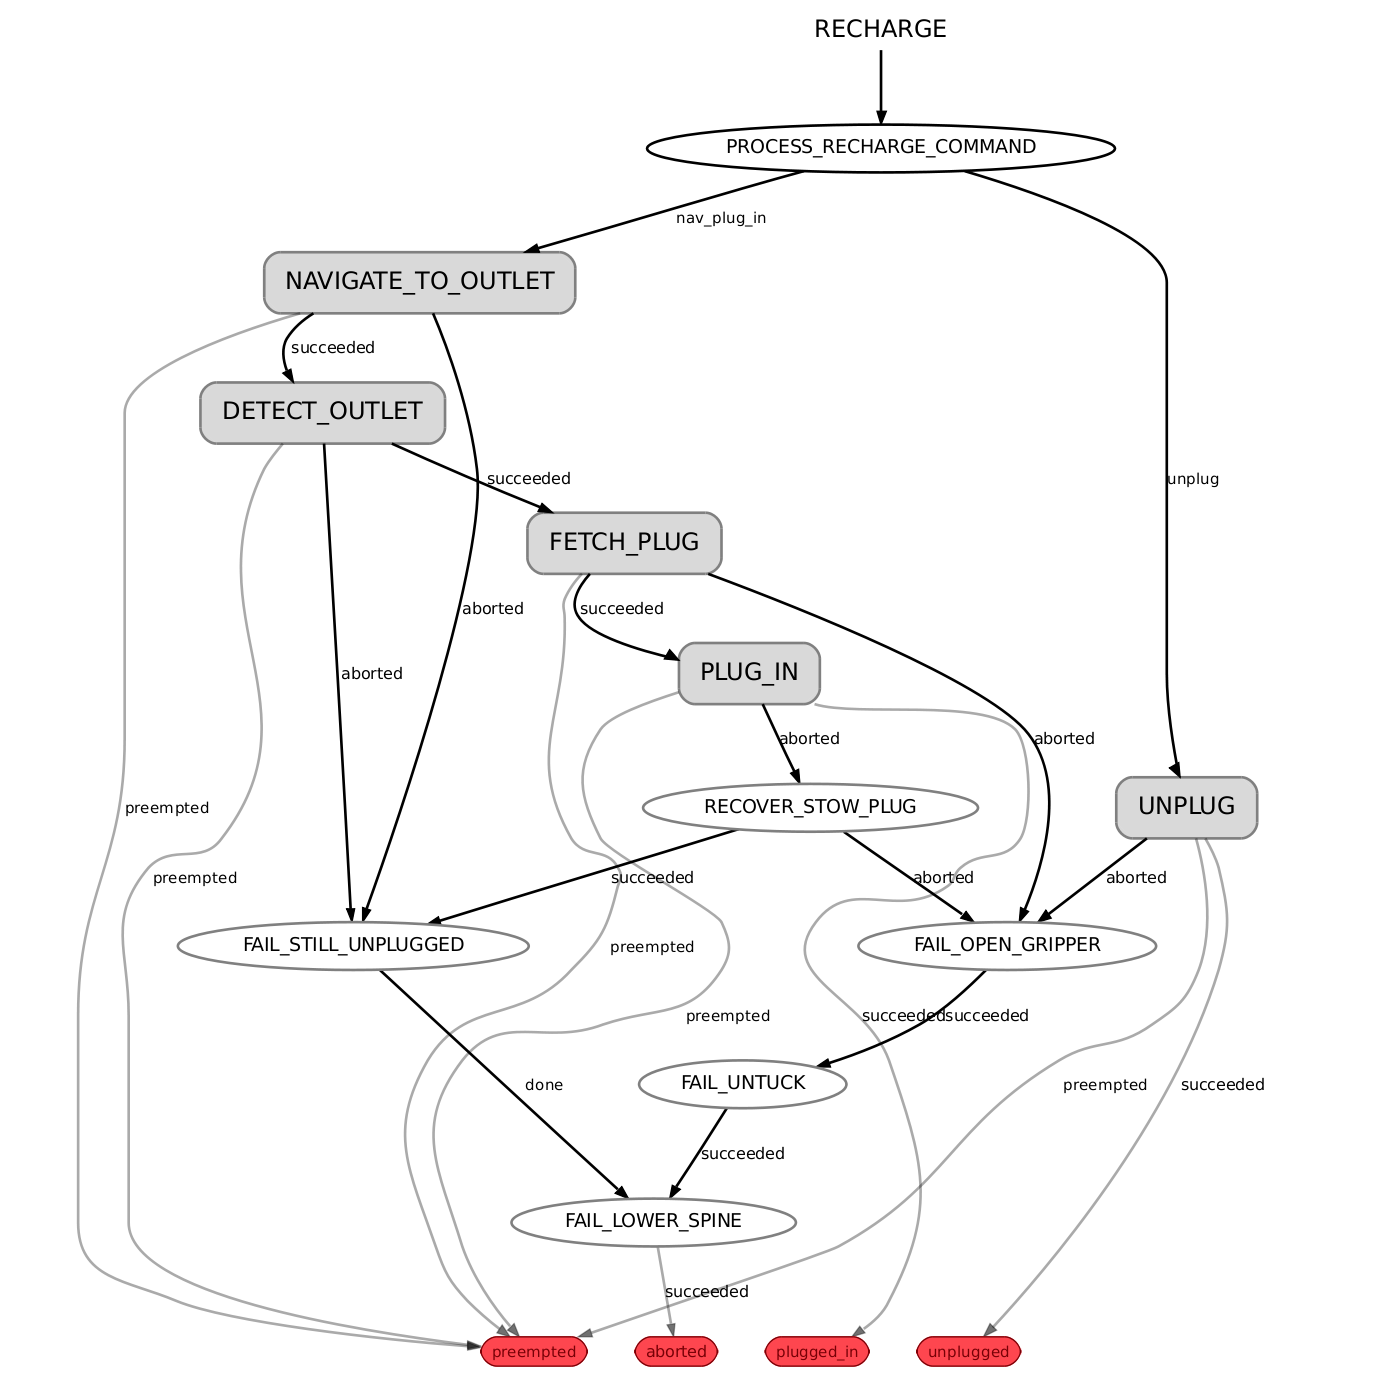
\includegraphics[width=0.8\textwidth]{smach-sample.png}
	\caption{\small Ejemplo de máquina de estado construida en SMACH para la representación de una rutina de carga automática de baterías. Obtenido desde la documentación oficial.}
	\label{img:SMACH-sample}
	\todounsure{Es necesario poner la figura en español??}
\end{figure}



En SMACH una maquina de estado está compuesta por un conjunto de estados y sus transiciones. La librería soporta anidamiento, por lo que cualquier estado puede ser reemplazado por otra máquina de estado disponible. Cada estado debe proveer una función \texttt{execute} a ser ejecutada cuando esté activo. En la Figura \ref{img:SMACH-sample} se presenta un ejemplo de un comportamiento robótico complejo implementado en SMACH, que representa el proceso de recarga de baterías en un robot. Según las condiciones encontradas se activarán distintas transiciones, pero en el caso básico la rutina es la siguiente: El robot navega a la estación de carga, se posiciona, manipula el conector, se conecta y espera.

%% =============================================================================
%% =============================================================================
%% =============================================================================
\subsection{UChile ROS Framework}\label{sec:URF}
%% =============================================================================
%% =============================================================================
%% =============================================================================

\subsubsection{Conceptos}

UChile ROS Framework (URF) hace referencia al sistema de software desarrollado en el laboratorio de robótica del Departamento de Ingeniería Eléctrica de la Universidad de Chile, para sus robots de servicio. El sistema cuenta con 10 años de desarrollo y está orientado a cumplir los requisitos de la competencia RoboCup en su categoría @Home.

URF está construido sobre ROS y en una estructura de 4 capas:
\begin{enumerate}
\item La primera capa contiene todas las dependencias del sistema, ya sean de ROS o no. Es la única capa que contiene sólo código externo.
\item  Sobre la primera capa se monta una capa ROS de bajo nivel, con herramientas y librerías comunes, sumado a los drivers necesarios para manejar cada robot (módulos de \textit{Hardware} en la Figura \ref{img:URF}).
\item La capa intermedia alberga capacidades robóticas avanzadas, relacionadas a percepción robótica, manipulación de objetos, navegación autónoma e interacción Humano-Robot (sección \textit{Módulos ROS} del diagrama).
\item La última capa \textit{de alto nivel} es desarrollada en Python, con interfaces para el uso de las capacidades de menor nivel, y es utilizada para la elaboración de maquinas de estado y comportamientos robóticos complejos mediante SMACH (cuadros \textit{Interfaz ROS-python} y \textit{State Machine} del diagrama).
\end{enumerate}

\begin{figure}[!h]
	\centering
	\includegraphics[width=0.8\textwidth]{URF-esp.png}
	\caption{\small Diagrama de UChile ROS Framework utilizado en el robot Bender.}
	\label{img:URF}
\end{figure}

Todos los módulos de URF son de código libre, a excepción de los algoritmos relacionados con percepción y la interfaz de alto nivel. El código se almacena públicamente en la organización \textit{uchile-robotics} en GitHub\footnote{Organización \textit{uchile-robotics} y URF en GitHub: \url{https://github.com/uchile-robotics}}.


\subsubsection{Memoria a corto y largo plazo}
%% =============================================================================

En un robot implementado sobre URF es posible acceder a la información compartida por sus procesos. Cualquier módulo ROS en el sistema tiene acceso a los datos extraídos desde sensores y luego generados en post-procesamientos, junto al acceso para controlar el hardware.

Existen algunas formas de memoria implementadas en URF, comparables a los conceptos definidos para la memoria humana. También se pueden dividir en de corto y largo plazo:

Como STM, se puede definir como memoria de trabajo a todo el flujo de información presente durante la ejecución del robot. Lo que incluye datos sensados, procesamientos y acciones realizadas. Generalmente tales datos no son almacenados para posteriores ejecuciones.

A manera de LTM, se puede encontrar una memoria procedural, relacionada con todo el conocimiento almacenado que posee el robot para cumplir ciertas tareas. Caen en esta categoría: modelos para percepción robótica, modelos para reconocimiento de voz y patrones, bases de datos de movimientos precalculados para manipular objetos y acciones predefinidas que se utilizan para controlar el robot.

También se pueden encontrar especializaciones de memoria LTM semántica. Ejemplos de esto son: El mapa que se conoce del entorno, junto a los lugares y objetos anotados en él. Diccionarios con información anotada sobre entidades y sus características, cómo personas y objetos. Bases de datos con imágenes anotadas para el reconocimiento de objetos y personas. 

Sin embargo, en URF no existen formas de memoria emocional ni episódica de largo plazo. Luego, toda interacción realizada por los robots está limitada a la información obtenida desde el inicio al término de cada rutina.


%% =============================================================================
%% =============================================================================
%% =============================================================================
\subsection{Bender}
%% =============================================================================
%% =============================================================================
%% =============================================================================
%% -----------------------------------------------------------------------------

Bender es un robot humanoide creado el año 2007 en el laboratorio de robótica del Departamento de Ingeniería Eléctrica de la Universidad de Chile. El equipo UChile Homebreakers es el encargado de su desarrollo y  su objetivo es ser un mayordomo para el hogar, funcionando de manera autónoma para apoyar en tales labores \cite{uchile-robotics}.

En cuanto a actuadores, el robot cuenta con 2 brazos antropomórficos de 6 grados de libertad cada uno, una base móvil diferencial Pioneer 3-AT, un cuello que permite rotaciones en dos ejes cartesianos; pudiendo imitar gestos de asentimiento y negación, y finalmente, una cabeza que puede mostrar expresiones faciales mediante movimientos de su boca, orejas, cejas y cambios de colores alrededor de los ojos.

El robot cuenta con los siguientes sensores: un laser Hokuyo UTM-30LX, un laser Hokuyo URG-04LX-UG01, un micrófono M-Audio Producer USB y una cámara de profundidad ASUS Xtion Pro.

El software de Bender está basado en el framework URF. Su arquitectura de software utiliza  ROS para el manejo de componentes de bajo y medio nivel. La capa de alto nivel, escrita en python, se abstrae de ROS y permite la creación de comportamientos complejos mediante máquinas de estado. Todos los módulos que interactúan con sensores y actuadores están implementados en ROS.

\begin{figure}[!h]
	\centering
	\includegraphics[width=0.4\textwidth]{bender.png}
	\caption{\small Robot Bender en competencia RoboCup@Home 2015.}
	\label{img:bender}
\end{figure}

\todoimprove{Sobre la cantidad de paquetes ROS, nodos, tópicos y mensajes disponibles.}
\todoimprove{API a ocupar para acceder a datos del robot.}


%% =============================================================================

%% =============================================================================

%% =============================================================================

%% =============================================================================

%% =============================================================================

%% =============================================================================

%% =============================================================================
%% =============================================================================
%% =============================================================================
\section{Algoritmos y conceptos computacionales}
%% =============================================================================
%% =============================================================================
%% =============================================================================
\todounsure{TODA ESTA SECCIÓN PODRÍA SER ELIMINADA....????}
\todounsure{convex hull}
\todounsure{procesamiento de imágenes: degradación de streams}
\todounsure{Algs utilizados para emociones implementadas en robot}
\todounsure{Sistemas de coordenadas?? Frames?}




\chapter{Diseño}\label{chapter:diseno}

En este capítulo se revisa el diseño del sistema LTM implementado en el proyecto. Primero, se presentan todos los requerimientos de diseño y se elabora un conjunto de validaciones que permitirán guiar el diseño, implementación y posterior evaluación del proyecto. Mediante las siguientes 4 secciones se describe la arquitectura del sistema: Se revisa el diseño de los episodios, su estructura de datos y limitantes. Luego se estudia el diseño del modelo de datos para la memoria episódica y su relación con los componentes semánticos. En tercer lugar se presenta el diseño del servidor LTM y sus limitantes. Finalmente, se definen la interfaz episódica y los componentes específicos a implementar para el robot Bender.

\todoimprove{Modificar ocurrencias de campos What, When, Where por versiones \texttt{What, When, Where}} 

%% =============================================================================
%% =============================================================================

%% =============================================================================
%% =============================================================================

%% =============================================================================
%% =============================================================================

%% =============================================================================
%% =============================================================================
\section{Requerimientos y validaciones}
%% =============================================================================
%% =============================================================================
%% =============================================================================

A continuación se presentan los requisitos de diseño sobre los que se construye el proyecto y las validaciones generadas a partir de ellos. Primero se da una descripción breve sobre el origen y razón de los requisitos. Luego, se presenta un listado formal de todos los requerimientos, escritos de una forma clara y verificable. Para concluir, se presenta un conjunto de pruebas que busca validar cada requerimiento expuesto.

%% =============================================================================
%% =============================================================================
%% ============================================================================= 
\subsection{Requisitos del proyecto}
%% =============================================================================
%% =============================================================================
%% =============================================================================

El primer conjunto de requisitos se deriva a partir de los objetivos del proyecto y sus alcances, presentados en la Sección \ref{sec:objetivos}.
\begin{itemize}
\item \RPlabelDef{1} Diseño de memoria de largo plazo episódica y semántica para robots de servicio domésticos, basado en los 11 requerimientos para una memoria episódica planteados por Stachowicz \cite{Stachowicz2012} y presentados en la Sección \ref{sec:ltm_exp}.
\item \RPlabelDef{2} Diseño debe considerar la modulación de los procesos cognitivos mediante memoria emocional.
\item \RPlabelDef{3} El diseño del sistema debe soportar el concepto de relevancia histórica.
\item \RPlabelDef{4} Además, los episodios deben manejar un indicador de relevancia generalizada, que encapsule todos los demás indicadores en sólo uno.
\item \RPlabelDef{5} Diseño del sistema debe ser agnóstico del robot a utilizar.
\item \RPlabelDef{6} El proyecto debe ser integrado en Bender, de manera no invasiva.
\end{itemize}


%% =============================================================================
%% =============================================================================
%% =============================================================================
\subsection{Requerimientos de sistema}
%% =============================================================================
%% =============================================================================
%% =============================================================================

Se desarrolló un documento (semiformal) de requisitos del sistema, derivados a partir de los requisitos de proyecto revisados en la sección anterior. Cada requisito de proyecto fue reformulado desde su versión difusa, uno o más requisitos de sistema precisos y verificables. El listado de puede ser encontrado en el Apéndice de Diseño, en la Sección \ref{appendix:req-sistema}.

El documento consta de 26 requisitos de sistema, cada una indicado por un prefijo y numeración de la forma \RSlabel{XX}. Cada uno indica su requisito de proyecto asociado. En el Apéndice \ref{chapter:appendix_a}, la Figura \ref{img:trazabilidad} muestra la matriz de trazabilidad de los requisitos de proyecto y sistema definidos.

%% =============================================================================
%% =============================================================================
%% =============================================================================
\subsection{Validaciones}
%% =============================================================================
%% =============================================================================
%% =============================================================================

También se desarrolló un documento (semiformal) con validaciones para cada uno de los requisitos de sistema en el documento. Las validaciones sirven como guía para la implementación del proyecto, y sus resultados son presentados y estudiados en el Capítulo \ref{chapter:results}. El listado completo se encuentra en el Apéndice de Diseño, en la Sección \ref{appendix:validations}.

Las validaciones fueron separadas en 5 categorías: 
\begin{enumerate}
	\item \Vlabel{A}{XX} Se verifican directamente desde el diseño e implementación del sistema.
	\item \Vlabel{B}{XX} Verificadas mediante la ejecución del sistema.
	\item \Vlabel{C}{XX} Validaciones de consultas LTM al servidor.
	\item \Vlabel{D}{XX} Validaciones de eficiencia
	\item \Vlabel{E}{XX} Validaciones de escalabilidad.
\end{enumerate}

El documento consta de alrededor de 35 validaciones, cada una indicada por un prefijo y numeración de la forma {\bfseries VTXX} (V: Validación, T: Tipo, XX: numeración). Cada validación indica su requisito de sistema asociado. En las Figuras \ref{img:trazabilidad-VA}-\ref{img:trazabilidad-VB}-\ref{img:trazabilidad-VC} se presentan matrices con el mapeo entre requisitos de sistema y las validaciones definidas.

Las validaciones \Vlabel{D}{XX} tienen por objetivo medir la eficiencia del sistema, una vez integrado en Bender. Se construyen a partir del requisito de sistema \RSlabel{15}. Cada una busca medir el uso de algún recurso del sistema, mientras el servidor se encuentra en funcionamiento y en espera. 

Las validaciones \Vlabel{E}{XX} se construyen a partir del requisito de software \RSlabel{16}. Tienen por objetivo medir el costo en tiempo de las operaciones de inserción, búsqueda y borrado de episodios, en función de la cantidad de episodios almacenados en la base de datos.


%% =============================================================================
%% =============================================================================

%% =============================================================================
%% =============================================================================

%% =============================================================================
%% =============================================================================

%% =============================================================================
%% =============================================================================
%% =============================================================================
\section{Diseño de episodios}
%% =============================================================================
%% =============================================================================
%% =============================================================================

A continuación presentan las decisiones de diseño seguidas para la representación de los datos episódicos mediante mensajes de ROS. Se estudia el formato a utilizar para el almacenamiento de cada episodio, seguido de la estructura de datos tipo árbol que soporta sus anidamientos. Luego se explica el diseño de los campos episódicos (\textit{What, When, Where}), la representación de la memoria semántica y el manejo de relevancias episódicas. Finalmente, se introducen los metadatos asociados a cada episodio y las limitantes del diseño episódico desarrollado para la representación episódica.

\todoimprove{AGREGAR DIAGRAMA GENERAL DEL SISTEMA... DB -- LTM -- PLUGINS -- USER}
\todoimprove{Agregar diagrama explicando anidamiento, transposición.}

%% =============================================================================
%% =============================================================================
%% =============================================================================
\subsection{Formato y representación}
%% =============================================================================
%% =============================================================================
%% =============================================================================

% SOBRE ELECCIÓN DE MENSAJES DE ROS
\paragraph{Mensaje ROS:}
Se decidió utilizar mensajes de ROS para la representación de episodios. Esto se justifica en la amplia gama de mensajes preconstruidos que provee, los que permiten generar un mensaje adecuado a cualquier necesidad. Además, al utilizar éste sistema de mensajes, se evita definir una formato de información particular para la representación episódica, y la comunicación de episodios mediante la API ROS del servidor se simplifica. Más aún, como se explicará en más detalle en la Sección \ref{}, el driver para MongoDB a utilizar permite almacenar cualquier estructura de datos, mientras ésta esté encapsulada en un mensaje ROS.

% SOBRE UNICIDAD
\paragraph{Unicidad:}
El requisito de software \hl{(RSXX)} exige que cada episodio sea único. Para esto, el mensaje ROS debe contener un campo que identifique al episodio. El servidor debe encargarse de que cada nuevo episodio cuente con un identificador único.

% SOBRE CAMPO DE TAGS
\paragraph{Tags:}
Además, para simplificar la búsqueda y reconocimiento de episodios, se incluye un campo de \textit{tags}. Éste corresponde a un vector de \textit{strings} y permite almacenar descripciones breves sobre la naturaleza del episodio. Por ejemplo, un episodio podría contener los siguientes \textit{tags}: ``cumpleaños'', ``fiesta'', ``atender invitados'' y ``torta''.

 
%% =============================================================================
%% =============================================================================
%% =============================================================================
\subsection{Árboles de episodios}
%% =============================================================================
%% =============================================================================
%% =============================================================================

\todounsure{Quitar manejo de contexto del trabajo??... no se si vale la pena que el server maneje ese concepto. Puede ser trabajo futuro.}

\todounsure{Es correcto hablar de hojas y nodos??... Debo buscar una palabra más adecuada para nodos que no son hojas??.. o debo explicitar que en adelante, cualquier referencia a nodo se refiere a eso. Suena raro hablar de ``padres''.}
\todowrite{Nodo == Nodo interno}

% SOBRE ANIDACIÓN Y ÁRBOLES EPISÓDICOS
\paragraph{Anidamiento episódico:}
A partir del requisito de software \hl{(RSXX)}, se debe soportar el concepto de anidación episódica. Este nace de la capacidad para expresar cualquier episodio, en términos de 1 o más sub-episodios más específicos. Para ello, se definen los \textit{árboles de episodios}, utilizando una estructura de datos de árbol: Las hojas contienen todo episodio que el sistema identifica como no divisible, mientras que cada padre es una representación menos específica de lo sucedido.

% SOBRE TEMPORALIDAD
\paragraph{Temporalidad:}
Para el árbol episódico, es fundamental que cada episodio padre inicie antes que cualquiera de sus hijos, y termine después que todos ellos. 

% SOBRE MANEJO DE INFORMACIÓN EN PADRES E HIJOS
\paragraph{Estrategia de almacenamiento:}
Ya que un padre puede ser representado lógicamente por su conjunto de hijos, se decide utilizar una metodología de almacenamiento que no genere redundancia de información. Sólo las hojas del árbol son las encargadas de manejar la información semántica del episodio, lo que potencialmente corresponde a una gran cantidad de información. Asimismo, las hojas son encargadas de manejar la mayor cantidad de información episódica que sea posible. Las estrategias para esto serán explicadas en sus respectivas secciones. Por lo tanto, los nodos del árbol manejan poca información y la mayor parte de sus datos puede ser calculada recursivamente a partir de sus hijos y de manera automática por el servidor.

% SOBRE EL CONTEXTO
\paragraph{Noción de contexto:}
Es importante enfatizar que no basta que un episodio esté embebido temporalmente en otro para ser considerado un hijo. Pues a pesar de cumplir la condición de temporalidad, puede ocurrir el caso de que ambos episodios sean simultáneos, pero estén ligados a un contexto distinto. Por ejemplo, dado un episodio A (robot está participando la competencia RoboCup - días de duración) y un episodio B (durante la competencia, robot es utilizado para una tarea de uno de los estudiantes, lo que es considerado ajeno a la competencia); a pesar de que A contiene temporalmente a B, se puede decir que B pertenece a otro contexto y debe ser almacenado en un árbol distinto. Esta noción de contexto es importante, y es la razón por la que el servidor debe manejar una cantidad indefinida de árboles episódicos, cada uno identificado por su raíz. Debido lo anterior, cada episodio debe ser almacenado indicando quien es el padre asociado.

 
\todoimplementation{Se puede agregar condición de que hijos son ordenados por tiempo de inicio}
 
%% =============================================================================
%% =============================================================================
%% =============================================================================
\subsection{Contexto temporal: \textit{When}}\label{sec:design_ep_when}
%% =============================================================================
%% =============================================================================
%% =============================================================================

% SOBRE LOS REQUISITOS
\paragraph{Requisitos:}
De acuerdo al requisito de software \hl{(RSXX)}, los episodios deben almacenar información que indique su contexto temporal (\textit{When}), es decir, cuándo  sucedió. Para esto, la única información de interés a almacenar son los instantes de tiempo que indican el fin y el inicio del episodio.

\todoimplementation{Revisar o modificar implementación.. no estoy seguro como se están manejando los tiempos para los padres... lo lógico sería no ajustar los tiempos a los de los hijos, pues estos pueden no estar definidos hasta el final!... O agregarlo como limitante.}
% SOBRE MANEJO DE INFORMACIÓN
\paragraph{Estrategia de almacenamiento:}
En el caso de las hojas del árbol, basta utilizar los instantes de tiempo obtenidos al iniciar y finalizar el episodio. Sin embargo, para el caso de los \hl{nodos}, se pueden seguir dos estrategias: Utilizar los instantes de tiempo iniciales y finales percibidos, o calcular automáticamente los tiempos de inicio y fin para ajustarse a los hijos. A pesar de que la segunda opción suena razonable, está asumiendo que siempre existirá un hijo para cada instante de tiempo de vida del padre, lo que puede no ser cierto. Por lo tanto, se deben manejar cuidadosamente los valores de tiempo de los padres, para asegurar que no son sobre-escritos por sus hijos, y para asegurar que los padres siempre contienen temporalmente a cada hijo.


%% =============================================================================
%% =============================================================================
%% =============================================================================
\subsection{Contexto espacial: \textit{Where}}
%% =============================================================================
%% =============================================================================
%% =============================================================================

% SOBRE LOS REQUISITOS
\paragraph{Requisitos:}
De acuerdo al requisito de software \hl{(RSXX)}, los episodios deben almacenar información que indique su contexto espacial (\textit{Where}), es decir, dónde sucedió. A continuación se explican las decisiones de diseño consideradas.

% SOBRE DURACIÓN DE EPISODIOS Y VECTORES
\paragraph{Desplazamiento durante episodios:}
En primer lugar, dependiendo de la duración del episodio, el robot puede haber estado en más de un lugar durante ese tiempo. Esto no es válido sólo para episodios nodo, sino que también para hojas, cuando éstas representan acciones de desplazamiento del robot. Luego, es importante que cada episodio registre cada uno de los lugares en los que ha estado el robot. El listado de lugares debe ser almacenado ordenadamente y con la hora asociada a cada desplazamiento, lo que es importante por dos motivos: permite calcular la secuencia de movimientos para los padres, y permite reconstruir la ruta del robot durante cada episodio. Para ello, la posición del robot puede ser consultada periódicamente en busca de cambios, para almacenar sólo los instantes que indiquen movimiento.
\todoimplementation{Soportar más de 1 lugar semántico y coordenado para hijos.}


% SOBRE USO DE AMBAS OPCIONES: Lugares y coordenadas
\paragraph{Estrategias de almacenamiento:}
La información espacial puede ser manejada de dos maneras: se pueden almacenar los nombres de los lugares en donde el robot estuvo durante el episodio, o se puede almacenar la ubicación precisa del robot durante el episodio, mediante coordenadas relativas a un sistema coordenado predefinido. La decisión sobre cual sistema utilizar depende mucho del contexto en el cual funciona el robot. Por ejemplo, en el caso de Bender, hay ocasiones en donde sólo es posible conocer su ubicación respecto a un sistema coordenado, mientras que en otras oportunidades, sólo se tiene conocimiento verbal de ésta. Luego, ya que no existe un consenso sobre que opción es la mejor, y para evitar limitar la usabilidad del sistema LTM, se decidió dar soporte a ambas alternativas.
\todounsure{Todo todo todo debe estar en 3ra persona singular presente??? como hablo de decisiones pasadas??... según esto, corregir todos los párrafos.}

% OPCIÓN SEMÁNTICA
\paragraph{Estrategia 1 - Descripción:}
Los nombres de lugares en los que estuvo el robot durante el episodio pueden ser almacenados utilizando vectores de \textit{strings}. Considerando el ambiente en donde puede desempeñarse un robot de servicio doméstico, se decide almacenar esta información en dos niveles de profundidad. El primer nivel corresponde a una descripción específica de la ubicación del robot (ej., ``Comedor''), mientras que el segundo sirve para almacenar el nombre del área donde se encuentra la primera ubicación (ej., ``Casa de John''), junto a otras de similar tamaño semántico. En el caso de los episodios nodo, se ha decidido calcular automáticamente toda esta información, a partir de los episodios hijo.
\todoimplementation{Crear submensaje para Where.msg, que almacene: location, area, time}

% OPCIÓN COORDENADAS
\paragraph{Estrategia 2 - Coordenadas:}
Similarmente al caso anterior, las coordenadas de lugares son almacenadas en vectores de puntos, junto con su hora y sistema de coordenadas asociados. Además, para cada punto se debe almacenar el nombre del mapa en donde se define el sistema coordenado. Ya que el proyecto está orientado a robots de servicio doméstico, se ha decidido implementar solamente ubicaciones en 2 dimensiones, es decir, cada punto sólo considera 2 valores numéricos. En el caso de los padres se sigue la siguiente estrategia: las posiciones son obtenidas a partir de sus hijos, se agrega un campo para almacenar la envoltura convexa de todas las posiciones, y se agrega un campo indicando el centroide de ésta.
\todoimplementation{Modificar implementación para agregar soporte a más de un frame/mapa.}
\todoimplementation{Crear submensaje para Where.msg, que represente ubicación coordenada múltiple}

%% =============================================================================
%% =============================================================================
%% =============================================================================
\subsection{Memoria semántica: \textit{What}}
%% =============================================================================
%% =============================================================================
%% =============================================================================

% REQUISITOS
\paragraph{Requisitos:}
De acuerdo a los requisitos de software \hl{(RSXXX), (RSXXX)}, la memoria semántica (\textit{What}) ligada a un episodio permite describir `qué'' sucedió en él. Ésta debe poder  contener cualquier dato, por lo que no es posible establecer de antemano qué información y estructura debe ser utilizada, sino que ésto debe poder ser definido por el usuario. El requisito \hl{(RSXXX)} (regla de flexibilidad episódica) establece que cada episodio debe permitir crear nuevos datos semánticos o actualizar los ya existentes. El requisito \hl{(RSXXX)} (regla de perspectiva episódica) exige que al leer un episodio, éste pueda describir sus datos semánticos asociados, de acuerdo a la misma perspectiva que se tenía de ellos cuando el episodio fue ejecutado.


% SEPARACIÓN DE CONCEPTOS
\paragraph{Streams y entidades:} 
La memoria semántica maneja entidades conocidas por el robot e información sobre ellas. Por ejemplo, se puede definir la entidad ``persona'' y almacenar datos como su nombre, nacionalidad o la fecha de la última interacción registrada. Sin embargo, existe un tipo de información que no está asociada a alguna entidad en particular, correspondiente a datos en forma de flujos de información (\textit{streams}). Éstos permiten registrar secuencias de imágenes, sonido y otros conceptos basados en flujos de datos percibidos por el robot, especialmente los obtenidos directamente desde sus sensores. Otra característica de los \textit{streams}, es que a diferencia de las entidades, representan datos que no se desea actualizar posteriormente, pues almacenan una imagen de lo percibido en el instante, la que generalmente es invariable. Entonces, se decide separar la memoria semántica en dos componentes, \textit{streams} y entidades, lo que permite diseñar estrategias de procesamiento adecuadas al funcionamiento de cada uno.


% GENERALIZANDO MEMORIA SEMÁNTICA
\paragraph{Generalización:}
Ya que los contenidos a almacenar deben poder ser definidos por el usuario, se establecen las siguientes decisiones de diseño. En primer lugar, el usuario debe definir que información utilizará, mediante uno o más mensajes de ROS. Segundo, éstos mensajes deben tener un campo para almacenar un identificador único. Los episodios deben tener referencias al tipo del mensaje asociado y a sus identificadores únicos. Similarmente, cada mensaje definido debe tener un campo para almacenar el identificador único de su episodio relacionado. Lo anterior es válido tanto para \textit{streams} como entidades.

\todopaused{Episodio almacena tags para describir entidades y cambios?.}


% SOBRE PLUGINS
\paragraph{Sistema de plugins:}
Se decidió utilizar un sistema basado en \textit{plugins}, para manejar los mensajes ROS definidos por el usuario. El diseño del servidor LTM en la Sección \ref{} especifica que funcionalidades deben ser implementadas por \textit{plugins} destinados a \textit{streams} o entidades. De esta manera, se delega al usuario la implementación de los algoritmos para adquisición de información semántica y procesamiento de ésta.


% SOBRE STREAMS
\paragraph{Datos semánticos - Streams:}
Los \textit{streams} corresponden a flujos de datos generalmente invariables. Cada episodio puede estar asociado a uno o más \textit{streams}, y a su vez, cada \textit{stream} puede contener uno o más datos. El servidor debe proveer notificaciones para indicar el inicio y fin de un episodio, mientras que el usuario debe definir su estrategia para adquirir datos durante ese lapso de tiempo. Por ejemplo, en el caso de un \textit{stream} de imágenes representando la visión del robot, y cuyo fin sólo sea de visualización a futuro, el usuario podría almacenar una imagen cada 3 segundos. 

Según la cantidad de \textit{plugins} a utilizar y la periodicidad de recopilación de información, el espacio de disco requerido para almacenar los mensajes puede ser agotado rápidamente. Para solucionar esto hay 3 alternativas. En primer lugar, se puede expandir la memoria disponible, lo que no es una solución real. En segundo lugar, está el ``olvido'' de información, mediante la eliminación de datos antiguos (posiblemente previo respaldo en otra máquina) o eliminar datos intercaladamente. La tercera opción es la degradación de información, para lo que cada usuario debe implementar un algoritmo que disminuya el tamaño de sus mensajes (por ejemplo, disminuyendo la resolución o cantidad de las imágenes del episodio). Ya que las dos primeras opciones pueden ser ejecutadas manualmente por el usuario, se ha decidido utilizar la degradación de mensajes. Esta estrategia puede ser aplicada automáticamente a mensajes antiguos y de baja relevancia episódica.

\todoimplementation{LTM server con warning en texto y notificación inotify cuando quede poco espacio de disco (menor a X\%) (o se ha ocupado más de X GB) debido al server... configurable por usuario...}


% SOBRE ENTIDADES
\paragraph{Datos semánticos - Entidades:}
% - manejo de datos y relaciones para regla perspectiva
% - manejo de datos y relaciones para flexibilidad
.

\todoimplementation{Manejo de perspectiva y audit al requerir insertar episodio al medio (temporalmente) de otros ya existentes.}

\todopaused{Escribir tras tener primera implementación razonable}


%% =============================================================================
%% =============================================================================
%% =============================================================================
\subsection{Relevancia generalizada}
%% =============================================================================
%% =============================================================================
%% =============================================================================

% RELEVANCIA GENERALIZADA
\paragraph{Requisitos:}
De acuerdo a los requisitos de software \hl{(RSXX), (RSXX) y (RSXX)}, los episodios deben almacenar información de relevancia episódica. Estos indicadores son importantes al momento de buscar episodios, para poder ordenarlos de acuerdo a una medida de importancia, y así tener una pista sobre cuales enfocar la atención. El sistema debe soportar, al menos, la noción de relevancia histórica y emocional, considerando que en un futuro se podrían agregar otros indicadores de relevancia. También, el sistema debe proveer un indicador generalizado, capaz de representar la relevancia global del episodio, mediante un solo indicador numérico que unifique las sub-relevancias.


% MANEJO DE INDICADORES
\paragraph{Estrategia de almacenamiento:}
Entonces, se define la siguiente estrategia de almacenamiento. Cada tipo de indicador debe proveer un valor numérico en el rango $[0, 1]$, que represente la importancia del episodio de acuerdo a su perspectiva. Un valor de 0 significa que el episodio no es relevante, mientras que el valor 1 es utilizado para indicar que el episodio es muy importante. Utilizando el formato anterior, se construye el indicador de relevancia generalizada a partir de todas las sub-relevancias definidas para el episodio. Este indicador debe ser actualizado cada vez que una sub-relevancia sea modificada o ingresada.


% COMPUTO BASADO EN ALGORITMO X
\paragraph{Cómputo:}
Este proyecto sólo considera dos sub-indicadores, histórico y emocional, por lo que se decidió utilizar la metodología propuesta por \hl{XXX} \cite{} y explicada en la Sección \ref{}.
\todopaused{Escribir más cuando esté implementado}


%% =============================================================================
%% =============================================================================
%% =============================================================================
\subsection{Relevancia emocional}
%% =============================================================================
%% =============================================================================
%% =============================================================================

% RELEVANCIA EMOCIONAL
\paragraph{Requisitos:}
El requisito de software \hl{(RSXXX)} exige el manejo del concepto de relevancia emocional, como un medio para almacenar las emociones ``que tiene'' el robot durante un episodio, en conjunto a un indicador de la intensidad de éstas.


% ABSTRACCIÓN DEL SISTEMA DE EMOCIONES
% - sobre EMOCIONES VÁLIDAS
\paragraph{Abstracción del sistema emocional:}
Según se revisó en la Sección \ref{}, existen diversas sistemas emocionales para la generación de emociones. No existe una metodología única para el cómputo de emociones, por lo que cada sistema es alimentado con datos diferentes, utilizan algoritmos distintos y proveen salidas distintas. Debido a la generalidad esperada de este proyecto, la forma de representar la emoción es se abstrae del sistema emocional a utilizar. Para esto, en primer lugar se define un conjunto de emociones base, a partir del modelo emocional de Plutchik descrito en la Sección \ref{}, con las que se debe construir la emoción asociada al episodio, mediante una combinación de ellas. Luego, se decidió utilizar un sistema de plugins, para que el usuario defina cómo realizar la asignación desde las salidas de su sistema emocional, a la combinación de emociones base disponibles para un episodio. Es así, como la asignación emocional se puede  abstraer de la implementación y delegar al usuario encargado de la plataforma objetivo.


% CAMPOS REQUERIDOS
\paragraph{Estrategia de almacenamiento:}
En primer lugar, se define un conjunto de 8 emociones base para la representación emocional (alegría, confianza, miedo, sorpresa, tristeza, disgusto, enfado y anticipación). El diseño considera sólo el almacenamiento de la emoción más importante durante la duración del episodio, la que es asociada a una emoción del conjunto base. Luego, siguiendo el estándar definido para representación de relevancias, se agrega un valor numérico en el rango $[0, 1]$, para  indicar la intensidad de la emoción seleccionada. Para el caso de episodios nodo, el valor emocional es calculado automáticamente a partir de los hijos. Para esto, se utiliza un vector de 8 valores, destinados a cada una de las 8 emociones base, donde se almacena el valor máximo de cada emoción presentado por sus hijos.

% METADATOS
\paragraph{Metadatos:}
Además, para simplificar la introspección de episodios a futuro, se decide agregar metadatos para indicar: software emocional utilizado y su versión, conjunto de salidas registradas por el software emocional y sus valores de intensidad. Es importante enfatizar que estos datos sólo deben ser utilizados para introspección y no tienen influencia en el cálculo de ninguna relevancia.
\todolater{Actualizar esto en caso de modificar metadatos}


%% =============================================================================
%% =============================================================================
%% =============================================================================
\subsection{Relevancia histórica}
%% =============================================================================
%% =============================================================================
%% =============================================================================

% SOBRE RELEVANCIA HISTORICA
\paragraph{Requisitos:}
El requisito de software \hl{(RSXXX)} exige el manejo del concepto de relevancia histórica, como un medio para indicar la importancia de un episodio, según su edad en la base de datos. 

% ALMACENAMIENTO
\paragraph{Estrategia de almacenamiento:}
Siguiendo el estándar definido para representación de relevancias, se utiliza un valor numérico en el rango $[0, 1]$, para  indicar el estado de envejecimiento del episodio. Este valor siempre debe ser inicializado en 1, para decaer hacia 0 con el paso del tiempo.


% MANEJO AUTOMÁTICO DE DATOS HISTÓRICOS
\paragraph{Actualización automática:}
El valor de la relevancia debe ser manejado automáticamente por el servidor LTM. Existen diversas formas de actualizar este valor, pero tras una revisión bibliográfica, se decidió utilizar la siguiente estrategia. Se propone disminuir el indicador, según el algoritmo de decaimiento estudiado por XXX en \cite{} y presentado en la Sección \ref{}. Ya que se espera almacenar una gran cantidad de episodios, se propone actualizar el valor cada lapsos cada vez más espaciados en el tiempo (por ejemplo, primero cada 1 día, luego 1 vez a la semana, cada 1 mes, cada 1 año), lo que permite acotar el esfuerzo computacional dedicado a las actualizaciones.

\todopaused{Sobre la tasa de decaimiento histórica implementada.}


%% =============================================================================
%% =============================================================================
%% =============================================================================
\subsection{Datos para introspección}
%% =============================================================================
%% =============================================================================
%% =============================================================================

% SOBRE RAZONAMIENTO
\paragraph{Metadatos:}
El último conjunto de datos considerado para almacenar junto a cada episodio es denominado \textit{Metadatos}. Éstos no están ligados a algún requerimiento de software, por lo que no son formalmente necesarios, sin embargo, permiten almacenar datos útiles para la implementación LTM, y sirven para conocer información sobre el software utilizado para almacenar cada episodio. Los \textit{Metadatos} tienen como finalidad ser de utilidad al resolver problemas relacionados al software LTM, y para cuando los usuarios deseen conocer el contexto de software sobre el cual fue generado el episodio.


%% =============================================================================
%% =============================================================================
%% =============================================================================
\subsection{Limitantes y trabajo futuro}
%% =============================================================================
%% =============================================================================
%% =============================================================================

% SOBRE LIMITANTES DEL DISEÑO Y TRABAJO FUTURO

A continuación se presenta un conjunto de limitantes conocidas del diseño episódico desarrollado, las que pueden ser consideradas como parte del trabajo futuro del proyecto.

% SOBRE COMPLETITUD Y LAPSOS EN BLANCO..
\paragraph{Ausencia de hijos:} Este problema fue explicado parcialmente en la Sección \ref{sec:design_ep_when}, y aparece con padres cuyo rango temporal no es cubierto completamente por sus hijos. Cómo se verá en la Sección \ref{}, esto puede suceder cuando el usuario decide no almacenar algunos episodios hoja, pues los considera poco relevantes. El efecto de ésto, es que puede haber información no presente en los padres, al calcular sus datos a partir de sus hijos. Particularmente, esto sucede con la información para \textit{When}, \textit{What} y las relevancias episódicas. Se puede argumentar que, ya que el usuario considera que los subepisodios eran irrelevantes, entonces la información perdida también lo es. Sin embargo, por motivos de introspección, puede ser de interés almacenar los datos de \textit{streams} asociados a los periodos temporales perdidos.

\paragraph{Episodios de larga duración:}
A pesar de que el diseño del servidor permite episodios de duración indefinida, en la práctica, es raro que el robot funcione por periodos prolongados. Luego, los episodios cuyo fin es dar un contexto temporal a un árbol no pueden ser almacenados directamente (por ejemplo, cuando el robot está participando en una competencia de 4 días de duración). A pesar de lo anterior, el diseño permite la introducción manual de episodios de larga duración, sin tener que mantener en funcionamiento el robot durante todo el periodo.

\todoimplementation{COMO MANEJAR CONTEXTOS, PUES SE PUEDE REQUERIR SU INFORMACIÓN, INCLUSO DURANTE EL MISMO EPISODIO!!.. DEBEN SER ALMACENADOS UNA VEZ INSCRITOS Y SER CERRADOS MANUALMENTE.}


\todowrite{Limitante Where: En un futuro se podría agregar un 3er nivel de información, para almacenar info ultra específica, por ejemplo: ``al lado de la tele'', ``cerca del refrigerador''..}


% SOBRE UBICACIÓN
\todopaused{Depende de reimplementación del sistema de ubicación}

%       - ubicación 2D
%       - ubicación y frames
%       - ubicaciones de hojas con sólo un lugar... vs episodios con movimiento.
%       - padres mantienen con mismo frame y mapa de hijos


%% =============================================================================
%% =============================================================================

%% =============================================================================
%% =============================================================================

%% =============================================================================
%% =============================================================================

%% =============================================================================
%% =============================================================================
%% =============================================================================
\section{Diseño del modelo de datos}
%% =============================================================================
%% =============================================================================
%% =============================================================================
% - Diseño de Base de Datos:

Es esta sección se presentan las decisiones sobre el diseño de la base de datos a utilizar para el proyecto. En primer lugar, se revisan las consideraciones sobre la base de datos escogida: \textit{MongoDB}. Luego, se describe el manejo de mensajes episódicos y sus datos semánticos asociados, \textit{streams} y entidades.


%% =============================================================================
%% =============================================================================
%% =============================================================================
\subsection{Base de datos}
%% =============================================================================
%% =============================================================================
%% =============================================================================

% SOBRE SELECCIÓN DE MONGO DB
\paragraph{MongoDB:}
Según se explicó en la Sección \ref{}, la implementación del sistema LTM requiere el manejo de datos aleatorios, representados mediante mensajes de ROS que debe definir el usuario. Además, el sistema debe permitir modificar la representación de tales mensajes a futuro y soportar el almacenamiento de datos binarios. Por lo tanto, se requiere el uso de una base de datos no relacional, capaz de manejar cualquier mensaje definido en ROS. Para ésto, se decidió utilizar la base de datos no relacional \textit{MongoDB}, presentada en la Sección \ref{}. 

La decisión sobre el uso \textit{MongoDB} se basa en tres razonamientos principales. Primero, el driver ROS para ésta es considerado estable, al menos hasta el año 2023. \textit{MongoDB} es utilizado por la librería \textit{MoveIt} de ROS, de uso extendido en la comunidad, por lo que ya ha sido probada y está disponible en muchos robots de servicio domésticos. Finalmente, \textit{MongoDB} se ocupa actualmente en el robot Bender. Debido a lo anterior, esta elección minimiza problemas de dependencias y compatibilidad a futuro.

\todounsure{Es correcto hablar de drivers??.. debo hablar sobre controladores?..}


% SOBRE SEPARACIÓN DE COLECCIONES
\paragraph{Colecciones:}
Debido al funcionamiento del driver ROS para \textit{MongoDB}, se asociará una colección distinta para cada mensaje episódico de interés. Particularmente, una colección será destinada al almacenamiento del mensaje \texttt{Episode.msg}, mientras que cada mensaje definido por el usuario será  asociado a una colección distinta. En primera instancia, la base de datos no relacional permitiría almacenar todos los mensajes en la misma colección, pero la separación de cada tipo de dato en colecciones distintas es conveniente debido a lo siguiente. Primero, la separación permite optimizar consultas simples a la base de datos, que no requieran acceder a toda la memoria semántica asociada. Además, mediante la separación se evita propagar problemas al registro de episodios, cuando se presenten fallos en los controladores de memoria semántica que debe implementar el usuario. Finalmente, ya que el sistema debe soportar una cantidad indefinida de mensajes ROS elegidos por el usuario, se evita saturar el registro de episodios con mensajes que, una vez agrupados, superen el límite de tamaño permitido a cada elemento de una colección.

% REQUISITO DE MODIFICACIÓN DE REPRESENTACIÓN
% modificar msg de colección MD5 y poder seguir ocupando la base de datos.
% - mongo no tiene problema en modificar representación ...
% - el driver ROS si.
.
\todopaused{Describir cuando esté solucionado.}


%% =============================================================================
%% =============================================================================
%% =============================================================================
\subsection{Colección de episodios}
%% =============================================================================
%% =============================================================================
%% =============================================================================

Toda la información episódica, definida por medio del mensaje \texttt{Episode.msg}, será almacenada en la colección \texttt{episodes}.

Debido a los requisitos de software \hl{(RSXX) y (RSXX)}, cada episodio debe ser indexado por todos sus campos disponibles, propuestos en la Sección \ref{}. Sin embargo, por temas prácticos, no es posible indexar todos los datos asociados al campo \textit{What}. En el caso de entidades, queda a criterio del usuario. Mientras que en el caso de \textit{streams}, no tiene sentido indexar cada pixel de una imagen, o cada instante de sonido a almacenar.


% SOBRE CONSULTAS QUE DEBE SOPORTAR?
\todowrite{Sobre consultas episódicas que debe soportar el modelo.}


%% =============================================================================
%% =============================================================================
%% =============================================================================
\subsection{Colecciones de streams}
%% =============================================================================
%% =============================================================================
%% =============================================================================

Según se explicó anteriormente, cada \textit{stream} definido por el usuario es asociado a una colección de \textit{MongoDB} propia. El nombre de la colección debe ser definido por el usuario. 

Ya que los \textit{streams} se consideran datos con sólo una instancia por cada episodio, se decide utilizar el mismo identificador único para ambas estructuras. Así, el episodio identificado por el valor $A$, tendrá asociado un \textit{stream} de cada colección, cada uno con el identificador $A$.

\todoimplementation{Que el server avise si hay colecciones con nombres repetidos.}

Por lo general, los campos de un \textit{stream} no requieren ser indexados, ya que es conveniente almacenarlos como campos binarios. Sin embargo, durante la implementación del \textit{plugin} asociado, el usuario puede decidir añadir metadatos para indexar campos convenientes. La utilidad de ésto, es que permitirá agregar nuevos términos de comparación para las consultas a la base de datos. Luego, se tienen dos formas de acceder a un \textit{stream} en particular; mediante su mensaje episódico asociado, o a través de los metadatos definidos por el usuario.

Utilizando la configuración por defecto de \textit{MongoDB}, el límite de tamaño para cada mensaje ROS a almacenar es de $16 MB$, lo que impone una cota superior a la cantidad de datos que pueden ser almacenados por cada episodio. Por ejemplo, esto permitiría almacenar $N$ imágenes a color de tamaño $AxB$, o $M$ imágenes en escala de grises del mismo tamaño. Sin embargo, \textit{MongoDB} provee estrategias de almacenamiento que no consideran esa limitante, las que deben ser configuradas por el usuario.
\todowrite{Corregir comparación de 16MB con cantidad de imágenes. Ojo con formato y serialización.}
\todoimplementation{Server con warning si mensaje a almacenar pesa más del límite!.}

% - cambio de representación (MD5)
\todopaused{Sobre la modificación de la estructura del stream... MD5...}


%% =============================================================================
%% =============================================================================
%% =============================================================================
\subsection{Colecciones de entidades}
%% =============================================================================
%% =============================================================================
%% =============================================================================

Cada mensaje ROS definido por el usuario, para representar una entidad de la memoria semántica, es  asociado a una colección de \textit{MongoDB} propia. El nombre de ésta debe ser definido por el usuario. 

A diferencia de los \textit{streams}, cada episodio puede estar asociado a una o más instancias de una entidad semántica. Por ejemplo, dada una entidad ``Persona'', durante un mismo episodio se pueden obtener datos (e.g., fecha de última visualización) para las instancias ``Jonh'' y ``Mike'', los que son almacenados en la misma colección, pero en distintas entradas.

\todoimplementation{Escribir cuando esté implementado correctamente.}

\todopaused{Sobre modelo de datos y flexibilidad...}
\todopaused{Sobre modelo de datos y perspectiva...}
% - cómo cumplir reglas sobre flexibilidad y perspectiva. Audit trail.

% SOBRE CONSULTAS QUE DEBE SOPORTAR?
\todowrite{Sobre consultas episódicas que debe soportar el modelo.}
\todopaused{Sobre metadatos}
\todopaused{Sobre tags definidos en campo What.}

% - cambio de representación (MD5)
\todopaused{Sobre la modificación de la estructura de entidades... MD5...}



%% =============================================================================
%% =============================================================================
%% =============================================================================
\subsection{Limitantes y trabajo futuro}
%% =============================================================================
%% =============================================================================
%% =============================================================================

El modelo de datos descrito está diseñado para satisfacer los requerimientos de software del proyecto, sin embargo, los siguientes aspectos no son cubiertos por el diseño y se consideran trabajo futuro.

\todowrite{Identificar más limitantes}
% - otras funcionalidades de interés: bkp, migrate a otro robot, ...
% - metadatos de arreglos... por el driver ROS...
% - cosa MD5


%% =============================================================================
%% =============================================================================

%% =============================================================================
%% =============================================================================

%% =============================================================================
%% =============================================================================

%% =============================================================================
%% =============================================================================
%% =============================================================================
\section{Diseño del servidor LTM}
%% =============================================================================
%% =============================================================================
%% =============================================================================
%    - TODO: manejo de contexto
.
\todowrite{Escribir descripción de la sección.}

% revisar requerimientos software asociados.

%% =============================================================================
%% =============================================================================
%% =============================================================================
\subsection{Manejo de episodios}
%% =============================================================================
%% =============================================================================
%% =============================================================================
% - Diseño del servidor LTM según requisitos
% - uso de MongoDB
% - Minimizar dependencias
% - API ROS: servicios, parámetros, nodos
% - parámetros (dar énfasis en la implementación)
% - estrategia de actualización episódica... branching.. etc.
.

\subsubsection{Interfaz episódica}
%% =============================================================================
% - proveer tiempo y anidamiento
% - permite notificar a los otros componentes para la recopilación de información episódica


%% =============================================================================
%% =============================================================================
%% =============================================================================
\subsection{Sistema de plugins}
%% =============================================================================
%% =============================================================================
%% =============================================================================
% - Sistema de plugins para agregar cosas específicas a cada robot
%    - where, emociones, streams y entidades.
%    - sobre información disponible para cada plugin
%    - requerimientos para cada plugin
%    - uso esperado de pluginlib
%    - flujo de trabajo de cada plugin
%    - se recomienda que sólo estén en funcionamiento cuando hay episodios registrados pendientes.
%    - sobre estabilidad de plugins.
.

\subsubsection{Plugin: \textit{Where}}
%% =============================================================================
% SOBRE: Funcionamiento recomendado del plugin
% - recopilación constante de posicionamiento del robot.
% - provee listado de poses dado tiempos de inicio, fin de episodio.
% - sólo recopila información cuando hay episodios registrados.
.

\subsubsection{Plugin: Emociones}
%% =============================================================================

% SOBRE: funcionamiento recomendado del plugin
% - recopilación de emociones .. buffer
% - provee emoción más fuerte del periodo.
% - rellenar metadatos 
% - sólo recopilar info si hay episodios registrados.
.

\subsubsection{Plugin: \textit{Streams}}
%% =============================================================================

% SOBRE: requerimientos del server
% - sobre marcar inicio, fin
% - sobre definición de colección
% - sobre manejo de la colección: CRUD
% - sobre API ROS asociada.
.

\subsubsection{Plugin: Entidades}
%% =============================================================================

% SOBRE: requerimientos del server
% - sobre marcar inicio, fin
% - sobre definición de colecciones
% - sobre manejo de la colección: CRUD
% - sobre API ROS asociada.
.

%% =============================================================================
%% =============================================================================
%% =============================================================================
\subsection{Alcances y trabajo futuro}
%% =============================================================================
%% =============================================================================
%% =============================================================================
%    - Alcances y trabajo futuro
%        - reservar ids mientras nodo esté activo.
%        - posibles funcionalidades de interés: 
%           - visualizador
%           - 
 .

%% =============================================================================
%% =============================================================================

%% =============================================================================
%% =============================================================================

%% =============================================================================
%% =============================================================================

%% =============================================================================
%% =============================================================================
%% =============================================================================
\section{Diseño de módulos específicos para Bender}
%% =============================================================================
%% =============================================================================
%% =============================================================================

Según especifica el requisito de software \hl{(RSXX)}, el proyecto debe ser integrado al robot Bender, con una demostración de las capacidades del sistema LTM. Para esto, se deben implementar módulos de software que permitan recolectar todos los datos episódicos requeridos por el servidor. A continuación se describe el diseño de los componentes a implementar: la interfaz para recolectar episodios, la posición del robot y sus emociones, junto a los plugins para la recolección de streams y entidades a partir de la memoria de trabajo. 

Cada uno de los módulos presentados a continuación cumple una doble funcionalidad. En primer lugar, cumplen con el requisito del diseño de componentes orientados a robots de servicio doméstico, enfocados en el robot Bender. Y además, sirven como ejemplo para el diseño e implementación de nuevas funcionalidades requeridas a futuro para otras plataformas.

%% =============================================================================
%% =============================================================================
%% =============================================================================
\subsection{Recolección de episodios: SMACH}
%% =============================================================================
%% =============================================================================
%% =============================================================================

\paragraph{SMACH:}
El módulo específico más importante a implementar corresponde al encargado de generar episodios a partir del funcionamiento del robot, para luego entregarlos al servidor LTM. Como se explica en la Sección \ref{}, en Bender se utiliza la librería SMACH para la definición y ejecución de las máquinas de estado encargadas de encadenar rutinas simples, para generar comportamientos complejos. A través de SMACH, en Bender se implementan capacidades como la interacción continuada con humanos y la resolución de tareas en el hogar. 

\paragraph{Información episódica:}
A partir de SMACH se puede obtener parte del conocimiento episódico requerido para la definición de un episodio. Desde el punto de vista de sus transiciones, las máquinas de estado están estructuradas en forma de grafo, estableciendo un inicio y fin temporal para cada estado. Conceptualmente, las máquinas se estructuran en forma de árboles, donde cada maquina de estado puede ser contenida por otra, lo que representa el anidamiento episódico. Luego, SMACH provee una forma de conocimiento episódico, capaz de representar información temporal (\textit{When}) y las relaciones de anidamiento episódico (referencias padre-hijo). Finalmente, ya que cada máquina de estado está asociada a una capacidad o contexto, se puede utilizar esa información para obtener los \textit{tags} requeridos para marcar cada episodio.

\paragraph{Funcionamiento:}
La interfaz episódica diseñada tiene 2 etapas importantes. En primer lugar, el durante la programación de la máquina, el desarrollador debe indicar que estados considera almacenar como episodio, en caso que sean ejecutados. Además, se deben para cada estado marcado, se debe indicar una lista de \textit{tags} que describan brevemente el estado. La segunda etapa ocurre durante el funcionamiento de la máquina de estado; Al inicio de cada estado, la interfaz debe registrar el episodio en el servidor e indicar el identificador de su estado padre, para recibir el identificador generado para tal estado. Al fin de cada episodio, debe notificar el cierre al servidor, para que éste ejecute las rutinas de recopilación de datos y almacene el episodio.


\paragraph{Estabilidad de la implementación:}
La ejecución ininterrumpida de SMACH durante una rutina crucial para el desempeño del robot. Si la librería deja de funcionar repentinamente o se detiene continuamente, el robot se detendrá o tomará mucho tiempo en realizar sus tareas, lo que durante una competencia puede tener pésimas consecuencias para el equipo. Es por esto, que la implementación de la interfaz entre el servidor LTM y SMACH debe ser estable. Particularmente, es de vital importancia que el funcionamiento de SMACH no se vea afectado por la implementación, independientemente de si ésta tiene problemas en su ejecución. 


\paragraph{Intrusividad:}
Por otro lado, la implementación debe minimizar las modificaciones a la librería SMACH y a las máquinas de estado ya implementadas. En primer lugar, si se modifica la librería SMACH, el equipo tendrá que agregar una copia de ésta y mantenerla a futuro, para lo que no hay personal ni tiempo suficiente. Segundo, el robot dispone de muchas máquinas de estado, las que deberán ser actualizadas para agregar la funcionalidad de la interfaz episódica. Por lo tanto, se toman las siguientes decisiones:
\begin{itemize}
\item La librería SMACH no puede ser modificada para la implementación de la interfaz.
\item Las modificaciones a las máquinas de estado deben ser mínimas y opcionales. Esto permitirá ir agregando soporte LTM de manera gradual al robot.
\end{itemize}


%% =============================================================================
%% =============================================================================
%% =============================================================================
\subsection{Recolección de dato episódico: \textit{Where}}
%% =============================================================================
%% =============================================================================
%% =============================================================================

% SOBRE plugin
Se debe implementar un plugin para Bender capaz de proveer la posición del robot durante cada episodio, según los requerimientos especificados en la Sección \ref{}. Por motivos prácticos, se consideran dos versiones a implementar, una con información falsa, y otra capaz de obtener datos reales desde el robot.

% SOBRE: Plugin con información Dummy
La versión ``de prueba'' debe proveer datos generados aleatoriamente para cada uno de los campos del mensaje \texttt{Where.msg}. La motivación para esto, es poder realizar pruebas durante la implementación del sistema y poder ejecutar validaciones que no precisen de la ubicación real del robot. Además, el plugin permite minimizar el uso del robot real para la implementación y validación del proyecto, pues el robot es un recurso compartido en el equipo de trabajo y su uso implica costos altos en términos de tiempo.

% SOBRE: Interfaz con robot Bender.
La segunda versión debe ser integrada en el software del robot, a través de la API para la obtención de su ubicación. Se utilizará la estrategia de funcionamiento recomendada en la Sección \ref{}. El plugin deberá recopilar información periódicamente para cada uno de los campos del mensaje \texttt{Where.msg}. Se deberá proveer un listado ordenado temporalmente de las ubicaciones recopiladas, cuando el servidor notifique el término del episodio. Para disminuir el uso de recursos, solamente se deben recopilar posiciones cuando hayan episodios registrados como pendientes en el servidor.
\todoimplementation{Plugin Where en Bender.}


%% =============================================================================
%% =============================================================================
%% =============================================================================
\subsection{Recolección de dato episódico: Emociones}
%% =============================================================================
%% =============================================================================
%% =============================================================================

% SOBRE: plugin
El siguiente plugin a implementar está encargado de proveer las emociones registradas por el robot durante cada episodio, según los requerimientos especificados en la Sección \ref{}. En este caso, también se consideran dos versiones a implementar, una que provee datos falsos, y otra capaz de obtener datos reales desde el robot. Ambas versiones deben recopilar datos para cada uno de los campos del mensaje \texttt{Emotion.msg}.

% SOBRE: plugin dummy
La versión ``de prueba'' debe proveer datos generados aleatoriamente para cada uno de los campos del mensaje \texttt{EmotionalRelevance.msg}. Similarmente al plugin para el campo \textit{Where}, este plugin permite realizar pruebas durante la implementación del sistema y ejecutar validaciones que no precisen de la emoción real del robot, mientras se minimiza el uso del robot. Sin embargo, la razón principal para su implementación es que actualmente el robot no cuenta con un sistema de emociones.

% SOBRE: Interfaz con robot Bender.
La segunda versión debe ser integrada con el software del robot, una vez que se haya implementado el sistema emocional en el robot. Para ésto, se utilizará la estrategia de funcionamiento recomendada en la Sección \ref{}. El plugin deberá recopilar información periódicamente sobre las emociones del robot. Una vez que el servidor notifique la finalización del episodio, el plugin debe proveer un mensaje \texttt{Emotion.msg} asociado a la emoción más intensa durante la duración de éste. Además, para disminuir el uso de recursos, solamente se debe recopilar información cuando hayan episodios registrados como pendientes en el servidor.

\todopaused{Hablar sobre el diseño de módulos emocionales para el robot}

\subsubsection{Modulo emocional: A}
%% =============================================================================

\subsubsection{Modulo emocional: B}
%% =============================================================================

\subsubsection{Modulo emocional: C}
%% =============================================================================

\subsubsection{Modulo emocional: servidor de emociones}
%% =============================================================================


%% =============================================================================
%% =============================================================================
%% =============================================================================
\subsection{Plugin para streams: Imágenes}
%% =============================================================================
%% =============================================================================
%% =============================================================================


% SOBRE: plugin
Para los plugins encargados de proveer streams de datos se escogió la recopilación solamente de imágenes. Bender dispone de variados datos en su memoria de trabajo que son candidatos para ser almacenados en la memoria semántica, como por ejemplo: el sonido percibido en su micrófono, las nubes de puntos 3D percibidas por su sensor de profundidad, o los posiciones de sus efectores. Sin embargo, el almacenamiento de imágenes es muy útil, pues sirve para la demostración final, permite visualizar lo sucedido en el episodio, y la implementación puede servir para otras plataformas, pues las cámaras de video son un sensor muy común en las plataformas robóticas domésticas. Por motivos prácticos, se consideran dos versiones a implementar, una con información ficticia y otra que recopila datos desde el robot real.

\todoimplementation{Proveer plugin agnóstico al robot, configurable a través de parámetros.}

Se utilizará la estrategia de funcionamiento propuesta en la Sección \ref{}, mediante el uso de un \textit{buffer} para almacenar las últimas imágenes percibidas. Luego, el plugin deberá entregar un vector con las imágenes asociadas al lapso episódico requerido. Además, el plugin deberá proveer una API para insertar, buscar, actualizar y borrar mensajes de la colección.
% - ... revisar implementación ...

% SOBRE: plugin dummy
La ``versión de prueba'' debe proveer imágenes obtenidas a partir de un archivo de video. Análogamente a los plugins anteriores, la motivación para esto, es poder acelerar la implementación del proyecto y poder ejecutar validaciones sin requerir el robot real.

% SOBRE Plugin a partir de cámara de cabeza.. una o dos cámaras...
La segunda versión debe ser integrada en el software robot, utilizando la API ROS para leer imágenes desde sus cámaras de video.

%% =============================================================================
%% =============================================================================
%% =============================================================================
\subsection{Plugins para entidades}
%% =============================================================================
%% =============================================================================
%% =============================================================================
%% =====================================================================================

Para los plugins encargados de definir entidades y recopilar sus cambios durante un episodio, se escogieron las entidades de ``Persona'' y ``Objeto''. Ésta selección fue realizada, pues son las entidades más utilizadas por el robot Bender, y probablemente las más significativas para todo robot de servicio doméstico. Otras entidades de alta relevancia que pueden ser consideradas como trabajo futuro, son las de ``Lugar'' y del ``Robot''. De manera similar al caso de los streams, se consideran dos versiones a implementar, una capaz de proveer información ficticia sobre cada entidad, y otra encargada de proveer información real recopilada por el robot.

\todopaused{Requiere implementación funcional de plugin para entidades.}


% SOBRE: requerimientos del server
% - sobre marcar inicio, fin
% - sobre definición de colecciones
% - sobre manejo de la colección: CRUD
% - sobre API ROS asociada.


% SOBRE: Funcionamiento
% - estrtategia de procesamiento
% - buffer
% - periodicidad
% - ... revisar implementación ...

% SOBRE: plugin dummy
% - motivación.. sirve para simulación y pruebas, sin tener acceso al robot.
% - generación de stream de imágenes a partir de un video

% SOBRE Plugin a partir de cámara de cabeza.. una o dos cámaras...
% - sobre eso, siguiendo estrategia definida.














\chapter{Implementación}\label{chapter:implementacion}

Es éste capítulo se describe la implementación del proyecto, a partir de las decisiones de diseño expuestas en el Capítulo~\ref{chapter:diseno}. Primero, se presenta la estructuración del software en términos de archivos y paquetes ROS. Luego se describe la implementación del sistema LTM: el modelo episódico, el servidor, el sistema de plugins y la API ROS para su utilización. En tercer lugar, se presentan módulos de software implementados para acelerar la implementación y validar el proyecto. Finalmente, se presenta la integración del sistema LTM en Bender, mediante su incorporación a URF.

% ==============================================================================
% ==============================================================================

% ==============================================================================
% ==============================================================================

% ==============================================================================
% ==============================================================================

% ==============================================================================
% ==============================================================================
% ==============================================================================
% ==============================================================================
\section{Estructura del software e instalación}
% ==============================================================================
% ==============================================================================
% ==============================================================================
% ==============================================================================

Esta sección presenta la estructuración del software implementado, en términos de sus archivos y paquetes ROS involucrados. Se describen las dependencias del proyecto, la estructura elegida para el sistema LTM, y la estructura para los plugins encargados de la recolección de información episódica.

\subsection{Dependencias}
% ==============================================================================
% ==============================================================================
% ==============================================================================

A continuación se describen todas las dependencias de software utilizadas para la implementación del proyecto. Éstas se dividen en las siguientes categorías: de sistema, del lenguaje \CC, del lenguaje Python y de ROS.


\subsubsection{Sistema}
% ==============================================================================

El proyecto fue desarrollado en Linux, Ubuntu 16.04. Las dependencias del sistema LTM son las siguientes:

\begin{itemize}
\item {\bfseries ROS kinetic}: Se utilizó la distribución \textit{kinetic} de ROS, la que cuenta con soporte hasta Abril del año 2021.
\item {\bfseries mongodb-server}: Paquete de software que contiene el servidor de MongoDB para Ubuntu 16.04.
\end{itemize}

La implementación del sistema debería ser compatible con versiones más recientes de ROS y Ubuntu, siempre que estén disponibles las dependencias mostradas en las siguientes secciones.


\subsubsection{Dependencias C$++$}
% ==============================================================================

El servidor fue implementado completamente utilizando \CC, bajo el estándar \CC03, que es soportado por la mayoría de los compiladores actuales y es el utilizado por defecto en ROS kinetic. A continuación se listan las dependencias de \CC \ utilizadas para la implementación del servidor.

\begin{itemize}
	\item {\bfseries mongo-cxx-driver}: Driver oficial para mongodb en \CC\footnote{Repositorio oficial de \texttt{mongo-cxx-driver}: \url{https://github.com/mongodb/mongo-cxx-driver.git}.}. 
	\item {\bfseries Boost Geometry}: Utilizado para el cómputo de la envoltura convexa y para el cálculo del centroide de un polígono.
\end{itemize}


\subsubsection{Dependencias Python}
% ==============================================================================

Se utiliza Python en su versión 2.7, que es el estándar utilizado para ROS kinetic. Las siguientes dependencias son sólo para los módulos específicos para la integración con Bender o para el software demostrativo.

\begin{itemize}
\item {\bfseries cv2}: Librería OpenCV 2. Utilizada para insertar imágenes ficticias en entidades\footnote{Página oficial de OpenCV: \url{https://opencv.org/}}. 
\item {\bfseries faker}: Librería utilizada para la generación de datos ficticios para entidades\footnote{Repositorio oficial de librería \texttt{faker} para Python: \url{https://github.com/joke2k/faker}}.
\end{itemize}


\subsubsection{Dependencias ROS}
% ==============================================================================

A continuación se listan las dependencias de paquetes ROS utilizados para la implementación del servidor.
\begin{itemize}
	\item Suite estándar de mensajes y servicios: std\_srvs, std\_msgs, geometry\_msgs, sensor\_msgs.
	\item {\bfseries pluginlib}: Librería estándar para la implementación de plugins en ROS.
\end{itemize}

Las siguientes dependencias son paquetes ROS utilizados para la implementación de componentes específicas para el robot Bender y para el software demostrativo.
\begin{itemize}
\item {\bfseries smach, smach\_ros}: Librería SMACH. Utilizada para la implementación de la interfaz episódica con máquinas de estado.
\item {\bfseries cv\_bridge}: Interfaz ROS con librería OpenCV. Utilizado para el manejo de imágenes en los plugins.
\end{itemize}


\subsection{Paquetes de software desarrollados}\label{sec:impl_packages}
% ==============================================================================
% ==============================================================================
% ==============================================================================

Con el motivo de separar conceptos e implementar un software independiente del robot objetivo, se separó la implementación en 6 paquetes ROS. El primero provee la conexión a la base de datos. El siguiente contiene solamente la implementación del servidor, otro provee plugins e interfaces episódicas genéricas, otro contiene código de ejemplo, para pruebas y validación. Los dos últimos contienen implementaciones específicas para el robot Bender.

Todos los paquetes de ROS implementados cuentan con un repositorio de software en GitHub, de carácter público.

\subsubsection{Paquete ROS: \texttt{ltm\_db}}
% ==============================================================================

El paquete se puede considerar un \textit{fork} de \texttt{warehouse\_ros\_mongo}. Extiende la versión original con nuevas funcionalidades para el manejo de colecciones en MongoDB, requeridas para la implementación del servidor LTM.

Particularmente, se agregaron las siguientes funcionalidades:
\begin{itemize}
\item Soporte para agregar arreglos como campos para ser indexados en colecciones. Los arreglos se pueden construir para los siguientes tipos de datos en \CC: \texttt{std::string}, \texttt{int}, \texttt{double} y \texttt{bool}. 
\item Soporte para metadatos anidados.
\item Soporte para arreglos de objetos como metadatos de una colección.
\item Soporte para búsquedas de mensajes en colecciones, mediante condición de pertenencia de valor a un arreglo.
\item Soporte para consultas genéricas basadas en el sistema de consultas de MongoDB. Se puede realizar cualquier consulta y combinación de condiciones, expresable en formato JSON, utilizando el estándar de consultas de MongoDB.
\end{itemize}

El paquete ROS se encuentra en un repositorio público en GitHub: \url{https://github.com/mpavezb/ltm\_db}.


\subsubsection{Paquete ROS: \texttt{ltm}}
% ==============================================================================

Contiene solamente la implementación del servidor y la documentación de éste. No se incluyen plugins ni interfaces episódicas, pues son consideradas como software no necesario o muy específico para un robot, como para ser considerado genérico. El paquete se puede encontrar en el siguiente repositorio público de software: \url{https://github.com/mpavezb/ltm}.


\subsubsection{Paquete ROS: \texttt{ltm\_addons}}
% ==============================================================================

Este paquete ROS implementa un plugin para adquisición de \textit{streams} de imágenes, junto a las interfaces para obtener episodios desde JSON y SMACH. Contiene software genérico, agnóstico del robot a utilizar. Los tres componentes anteriores pueden ser considerados herramientas útiles para algún robot, pero que no son estrictamente necesarios para el funcionamiento del sistema LTM. El repositorio asociado se puede encontrar en: \url{https://github.com/mpavezb/ltm\_addons}.


\subsubsection{Paquete ROS: \texttt{ltm\_samples}}
% ==============================================================================

Este paquete contiene implementaciones de ejemplo de algunos plugins episódicos capaces de generar información ficticia. Además, el paquete contiene software útil para pruebas del funcionamiento del sistema y código para su validación. Su repositorio de software se encuentra en: \url{https://github.com/mpavezb/ltm\_samples}.


\subsubsection{Paquete ROS: \texttt{bender\_emotion}}
% ==============================================================================

Ya que Bender no dispone de un software generador de emociones, este paquete implementa el sistema emocional descrito en la Sección~\ref{sec:design_bender}. El repositorio se encuentra alojado en la cuenta GitHub del equipo encargado de Bender: \url{https://github.com/uchile-robotics/bender\_emotion}.


\subsubsection{Paquete ROS: \texttt{bender\_ltm}}
% ==============================================================================

Este paquete implementa plugins específicos para el uso del sistema LTM en el robot Bender, y es considerado el punto de integración del proyecto con el robot. Similarmente al paquete \texttt{bender\_emotion}, su repositorio se encuentra alojado en: \url{https://github.com/uchile-robotics/bender\_ltm}.


\subsection{Líneas de código}
% ==============================================================================
% ==============================================================================
% ==============================================================================

En la Figura~\ref{table:lineas-codigo} se presenta una tabla con el conteo de líneas de código implementadas para el proyecto, ordenadas por el lenguaje utilizado. Se utilizó el programa \texttt{cloc}\footnote{Repositorio del programa \texttt{cloc} en GitHub: \url{https://github.com/AlDanial/cloc}} para realizar el cómputo.

\begin{figure}[!ht]
	\centering
	\begin{tabular}{|l|r|r|r|r|}
		\hline
		\rowcolor{gray!50}
		Lenguaje & Archivos & Líneas en blanco & Comentarios & Código \\ \hline
		C++                   &  32  &  669  &  422  &  3073 \\ \hline
		C/C++ Header          &  47  &  667  &  422  &  2192 \\ \hline
		Python                &  37  &  587  &  471  &  1812 \\ \hline
		JSON                  &  12  &    0  &    0  &   321 \\ \hline
		CMake                 &   5  &  107  &  219  &   312 \\ \hline
		XML                   &  17  &   91  &   79  &   213 \\ \hline
		Markdown              &   8  &   95  &    0  &   183 \\ \hline
		ROS msg/srv           &  30  &   34  &   72  &   177 \\ \hline
		BASH    &   2  &   21  &    7  &    99 \\ \hline
		YAML                  &   4  &   30  &   45  &    77 \\ \hline
		\rowcolor{gray!50}
		Total                 & 194  & 2301  & 1737  & 8459  \\ \hline	
	\end{tabular} 
	\caption[Líneas de código del sistema LTM por lenguaje.]
	{\small Líneas de código del sistema LTM por lenguaje.}
	\label{table:lineas-codigo}
\end{figure}


\subsection{Documentación}
% ==============================================================================
% ==============================================================================
% ==============================================================================

Todos los paquetes ROS desarrollados para el sistema LTM, junto a los módulos de ejemplo para recopilación de información ficticia y desde el robot Bender, se encuentran documentados en el archivo \texttt{README.md} del paquete ROS \texttt{ltm}.

La documentación incluye una guía de instalación del proyecto y sus dependencias, junto a ejemplos sobre el uso del servidor y la elaboración de plugins.


% ==============================================================================
% ==============================================================================

% ==============================================================================
% ==============================================================================

% ==============================================================================
% ==============================================================================

% ==============================================================================
% ==============================================================================
% ==============================================================================
% ==============================================================================
\section{Sistema LTM}
% ==============================================================================
% ==============================================================================
% ==============================================================================
% ==============================================================================

En esta sección se describe la implementación del sistema LTM desarrollado. Primero, se presenta el modelo de datos para la definición de episodios, \textit{streams} y entidades. Luego, se describe la implementación del servidor LTM, basada en la librería \texttt{pluginlib}. Se presenta el sistema de plugins desarrollado y sus requisitos para los usuarios. Finalmente, se presenta la API ROS que provee el sistema LTM, para su configuración, ejecución, recolección de episodios y realización de consultas al servidor.


\subsection{Modelo de datos}
% ==============================================================================
% ==============================================================================
% ==============================================================================

A continuación se presenta el modelo de datos, construido a partir de mensajes ROS, utilizado para manejar los conceptos de episodios, entidades y \textit{streams}. Los mensajes implementados son la base para la construcción del sistema LTM y definen la estructura episódica a utilizar para la comunicación entre los clientes y el servidor en ROS.

Todos los mensajes presentados a continuación se encuentran en el paquete ROS \texttt{ltm}.

\subsubsection{Episodios}

A partir del diseño propuesto en la Sección~\ref{sec:ep_design}, se construye el mensaje ROS \texttt{ltm/Episode.msg}\footnote{El dominio \texttt{ltm/} hace referencia al nombre del paquete ROS donde se implementa el servidor y que contiene la definición de todos los mensajes relacionados.}, presentado en el Código~\ref{lst:episode.msg}. El mensaje tiene campos para manejar la estructura de árbol episódico, la información sobre \textit{What}, \textit{When} y \textit{Where}, las relevancias episódicas, y la información para introspección.
\lstset{style=/Style/ROS/MSG}
\lstinputlisting[caption=ltm/Episode.msg,label=lst:episode.msg]{code/msg/Episode.msg}

Para ordenar la información, el mensaje se construye a partir de otros mensajes ROS definidos en el mismo paquete:
\begin{itemize}
\item \texttt{ltm/When.msg}: Mantiene el contexto temporal del episodio, indicando tiempos de inicio y fin, mediante campos del tipo \texttt{time}\footnote{El tipo de dato \texttt{time} es estándar en ROS y permite indicar un instante de tiempo mediante un contador de segundos transcurridos desde el tiempo cero (Jueves 1 de Enero de 1970 a las 00:00:00). Tiene una resolución de nanosegundos.}.
\item \texttt{ltm/When.msg}: Almacena el contexto espacial del episodio, utilizando dos estrategias.
\begin{itemize}
\item  Permite almacenar un conjunto de coordenadas, mediante mensajes del tipo \texttt{geometry\_msgs/Point.msg}\footnote{El paquete de ROS \texttt{geometry\_msgs} proporciona mensajes para manejar primitivas geométricas y sus transformaciones. Pertenece al conjunto de paquetes para mensajes \texttt{common\_msgs}, el cual se considera estable. Más información en la web oficial: \url{http://wiki.ros.org/geometry\_msgs}}, sumado al nombre del mapa y del sistema coordenado utilizado. Además, se mantiene la envoltura convexa de las posiciones de sus hijos.
\item Permite almacenar la ubicación del robot en formato textual.
\end{itemize}
\item \texttt{ltm/What.msg}: Almacena referencias a cada pieza de memoria semántica asociada al episodio. Se construye a partir de un mensaje para el manejo de \textit{streams} y otro para el manejo de entidades.
\begin{itemize}
\item \texttt{ltm/StreamRegister.msg}: Utilizado para mantener un listado de cada \textit{stream}, mediante su identificador único y el tipo de mensaje ROS registrado por su plugin.
\item \texttt{ltm/EntityRegister.msg}: Utilizado para mantener un listado de cada entidad asociada al episodio, mediante el tipo de mensaje ROS registrado por su plugin, su identificador único, y un listado de los registros ingresados en el historial de la entidad.
\end{itemize}
\item \texttt{ltm/Relevance.msg}: Almacena datos sobre la relevancia episódica generalizada y las sub relevancias.
\begin{itemize}
\item La relevancia generalizada es construida mediante un indicador numérico y la fecha de su última actualización.
\item \texttt{ltm/EmotionalRelevance.msg}: Almacena la relevancia emocional del episodio. Mantiene un indicador numérico para la emoción más relevante, los valores de cada una de las 8 emociones percibidas, sumado a información sobre el software emocional utilizado.
\item \texttt{ltm/HistoricalRelevance.msg}: Almacena la relevancia histórica del episodio. Mantiene un indicador numérico, la fecha de la última actualización y la fecha de la siguiente actualización agendada.
\end{itemize}
\item \texttt{ltm/Info.msg}: Utilizado para almacenar metadatos del episodio, útiles para una introspección posterior por parte del usuario. Mantiene información como la fecha de creación y de último acceso al episodio, e información sobre el sistema operativo, la versión de ROS y la versión del sistema LTM utilizada.
\end{itemize}
 
Todos los mensajes ROS descritos anteriormente se pueden encontrar en el Anexo de Implementación, en la Sección~\ref{appendixB:modelo_datos}.


\subsubsection{Construcción de \textit{streams}}

\ltmconcept{Metadatos}
Los \textit{streams} se definen a partir de mensajes ROS construidos por el usuario, Los que pueden contener cualquier estructura soportada por ROS para sus mensajes. La implementación impone solamente un requisito sobre su definición. Se debe añadir un campo de tipo \texttt{ltm/StreamMetadata.msg} al mensaje, bajo el nombre \texttt{meta}. El tipo \texttt{ltm/StreamMetadata.msg}, presentado en el Código~\ref{lst:streammetadata.msg}, contiene información manejada por el servidor, indicando los tiempos de inicio y fin del \textit{stream}, sumado a los identificadores del mensaje y su episodio asociado.
\lstset{style=/Style/ROS/MSG}
\lstinputlisting[caption=ltm/StreamMetadata.msg,label=lst:streammetadata.msg]{code/msg/StreamMetadata.msg}


\subsubsection{Construcción de entidades}

\ltmconcept{Metadatos}
En el caso de las entidades, se deben almacenar distintas instancias de la entidad, cada una asociada a su historial de cambios. Una entidad es definida a través de un mensaje ROS construido por el usuario, y puede contener cualquier estructura soportada por ROS para sus mensajes. De manera similar al caso de los \textit{streams}, cada mensaje debe contener un campo de nombre \texttt{meta} y tipo \texttt{ltm/EntityMetadata.msg}. Este campo es manejado por el servidor y permite identificar la instancia de la entidad, asociada al mensaje. El tipo \texttt{ltm/EntityMetadata.msg} se presenta en el Código~\ref{lst:entitymetadata.msg}.
\lstset{style=/Style/ROS/MSG}
\lstinputlisting[caption=ltm/EntityMetadata.msg,label=lst:entitymetadata.msg]{code/msg/EntityMetadata.msg}

\ltmconcept{Historial}
Como se describe en el diseño del modelo de datos (ver Sección~\ref{sec:data_model_design}), el historial se construye utilizando dos colecciones, de sufijos \texttt{.trail} y \texttt{.meta}. Cada mensaje almacenado en una colección tiene asociado un registro en la otra, bajo el mismo identificador. 

La colección de sufijo \texttt{.meta} se construye a partir de mensajes ROS de tipo \texttt{ltm/EntityLog.msg}, presentado en el Código~\ref{lst:entitylog.msg}. Este tipo de mensajes es manejado automáticamente por el servidor, y permite indicar lo siguiente: Identificadores de la instancia, del registro y de los episodios asociados. Instante de tiempo del registro. Registro que precede al mensaje (lista enlazada de registros). Nombres de campos que fueron agregados, modificados o eliminados.
\lstset{style=/Style/ROS/MSG}
\lstinputlisting[caption=ltm/EntityLog.msg,label=lst:entitylog.msg]{code/msg/EntityLog.msg}

La colección de sufijo \texttt{.trail} se construye a partir de mensajes ROS del mismo tipo definido por el usuario. El campo \texttt{meta} es utilizado para asociar bidireccionalmente cada entrada del historial, a su mensaje mensaje de tipo \texttt{ltm/EntityLog.msg} en la colección de sufijo \texttt{.meta}.
 

\subsection{Servidor}
% ==============================================================================
% ==============================================================================
% ==============================================================================

El servidor es implementado de acuerdo a las decisiones de diseño estudiadas en el Capítulo~\ref{chapter:diseno}, y su estructura se basa en el diagrama de la Figura~\ref{img:diagrama-software}. La implementación se realiza completamente en el lenguaje \CC y se encuentra en el paquete ROS \texttt{ltm}. El servidor sólo depende de tipos de dato primitivos y paquetes estándar disponibles en todas las distribuciones ROS (e.g. \texttt{geometry\_msgs} y \texttt{std\_msgs} y \texttt{pluginlib}), el módulo geométrico la librería Boost, y el driver para la base de datos. 

La implementación se puede separar lógicamente en 2 componentes: memoria episódica y memoria semántica. La primera se encarga de adquirir episodios a partir de la API episódica que provee el servidor, mientras que el componente semántico se encarga de los \textit{streams} y entidades, por medio de los plugins que define el usuario.

La base de datos es manejada automáticamente por el servidor, por lo que el usuario no tiene un acceso directo a ésta, sino que sólo puede realizar operaciones de escritura a través de la API ROS del servidor y de las facilidades que proveen los plugins. Todas las funcionalidades para el manejo de MongoDB se encuentran en el paquete ROS \texttt{ltm\_db}.


\subsection{Plugins}
% ==============================================================================
% ==============================================================================
% ==============================================================================

El diseño del sistema LTM requiere que el usuario implemente 4 tipos de plugins para la adquisición de información episódica y semántica. Por un lado, se debe implementar un plugin para la adquisición del estado emocional del robot, y un plugin para obtener la ubicación del robot durante cada episodio. Por otro lado, el usuario puede implementar una cantidad indefinida de plugins para la recopilación de información semántica (\textit{streams} y entidades) que requiera para su aplicación robótica.

La implementación utiliza el paquete ROS \texttt{pluginlib} para la definición y carga dinámica de plugins definidos en paquetes ROS externos. Además, ya que los mensajes ROS definidos por el usuario para \textit{streams} y entidades no son conocidos en tiempo de compilación, se hace uso intensivo de tipos de dato genéricos en \CC \ para su representación y el manejo de la base de datos. A continuación, se presentan las consideraciones para la implementación de cada tipo de plugin requerido.


\subsubsection{Plugins episódicos: \textit{Where} y Emociones}
% ==============================================================================

Estos dos plugins son necesarios para obtener información episódica dependiente del robot objetivo. El único requisito impuesto para el usuario, es la implementación de cada plugin mediante el estándar utilizado en \texttt{pluginlib}, para proveer cada dato episódico cuando el servidor lo requiera. Se aconseja seguir la estrategia de funcionamiento descrita en la Sección~\ref{sec:design-server}.

El plugin de emociones debe heredar la clase \texttt{ltm::plugin::EmotionBase}, definida en \texttt{\#include \textless ltm/plugin/emotion\_base.h\textgreater}. Se deben implementar los \textit{métodos virtuales} declarados en la clase padre.

De la misma manera, el plugin para recolectar el campo \textit{Where} debe heredar la clase \texttt{ltm::plugin::LocationBase}, definida en \texttt{\#include \textless ltm/plugin/location\_base.h\textgreater}. El plugin debe implementar los \textit{métodos virtuales} declarados por la clase padre.


\subsubsection{Plugins: \textit{Streams}}
% ==============================================================================

\ltmconcept{Plugin a implementar}
Se debe implementar un plugin por cada \textit{stream} definido por el usuario. Cada plugin debe heredar de la clase \texttt{ltm::plugin::StreamBase}, definida en \texttt{\#include \textless ltm/plugin/stream\_base.h\textgreater}. Se deben implementar los \textit{métodos virtuales} declarados por la clase padre. Las funcionalidades requeridas se describen en la Sección~\ref{sec:design_server_semantic_plugins} y se recomienda utilizar la estrategia de procesamiento propuesta en la misma sección.

\ltmconcept{Servicio ROS}
Además, ya que los plugins son cargados dinámicamente, el mensaje ROS definido por el usuario no es conocido en tiempo de compilación. Es por esto, que para proveer una API CRUD mediante servicios ROS, se requiere que el usuario defina un servicio adecuado a su mensaje. El archivo \texttt{.srv} debe tener el formato presentado en el Código~\ref{lst:samplestreamsrv}, donde \texttt{\textless user\_package\textgreater} y \texttt{\textless stream\_msg\textgreater} hacen referencia al paquete ROS y al tipo del mensaje definido por el usuario, respectivamente.
\lstset{style=/Style/ROS/MSG}
\lstinputlisting[caption=SampleStreamSrv.srv,label=lst:samplestreamsrv]{code/srv/SampleStreamSrv.srv}

\ltmconcept{Funcionalidades heredadas}
Dado que \texttt{pluginlib} no soporta clases base basadas en templates de \CC, el plugin debe heredar de la clase \texttt{ltm::plugin::StreamDefault\textless MsgType, SrvType\textgreater}, definida en \texttt{\#include \textless ltm/plugin/stream\_default.h\textgreater}, donde \texttt{MsgType} y \texttt{SrvType} deben ser reemplazados por la clase del mensaje y servicio ROS manejados por el plugin. Lo anterior, permite al plugin manejar automáticamente la base de datos y proveer una API CRUD mediante servicios ROS, adecuada al mensaje en cuestión y simplificando la implementación del plugin.


\subsubsection{Plugin: \textit{Entidades}}
% ==============================================================================

\ltmconcept{Plugin a implementar}
De manera análoga al caso de los \textit{streams}, se debe implementar un plugin por cada entidad definida por el usuario. Cada plugin debe heredar de la clase \texttt{ltm::plugin::EntityBase}, definida en \texttt{\#include \textless ltm/plugin/entity\_base.h\textgreater}. Se deben implementar los \textit{métodos virtuales} declarados por la clase padre. Las funcionalidades requeridas se describen en la Sección~\ref{sec:design_server_semantic_plugins} y se recomienda utilizar la estrategia de procesamiento propuesta en la misma sección.

\ltmconcept{Servicio ROS}
Para este tipo de plugin, también se requiere que el usuario defina un servicio adecuado a su mensaje. El archivo \texttt{.srv} debe tener el formato presentado en el Código~\ref{lst:sampleentitysrv}, donde \texttt{\textless user\_package\textgreater} y \texttt{\textless entity\_msg\textgreater} hacen referencia al paquete ROS y al tipo del mensaje definido por el usuario, respectivamente.
\lstset{style=/Style/ROS/MSG}
\lstinputlisting[caption=SampleEntitySrv.srv,label=lst:sampleentitysrv]{code/srv/SampleEntitySrv.srv}

\ltmconcept{Funcionalidades heredadas}
La implementación provee automáticamente funcionalidades para el manejo de la base de datos y una API CRUD mediante servicios ROS. Para ésto, el plugin a implementar debe heredar la clase \texttt{ltm::plugin::EntityDefault\textless MsgType, SrvType\textgreater}, definida en \texttt{\#include \textless ltm/plugin/stream\_default.h\textgreater}, donde \texttt{MsgType} y \texttt{SrvType} deben ser reemplazados por la clase del mensaje y servicio ROS manejados por el plugin.


\subsection{API ROS}
% ==============================================================================
% ==============================================================================
% ==============================================================================

A continuación se presenta la API ROS para el uso de las funcionalidades del sistema LTM implementado. Se explica el uso del servidor de parámetros de ROS para la configuración del servidor LTM, y el uso de la herramienta \texttt{roslaunch} para su ejecución. Luego, se presenta la API para recolección de episodios, a partir de servicios ROS. Finalmente, se presenta la API para realizar consultas episódicas y semánticas al sistema LTM.

Es importante destacar que a pesar de que el sistema se implemente en \CC, ROS permite utilizar todas las funcionalidades de la API a través de diversos lenguajes de programación: Nativamente en \CC  (\texttt{roscpp}), Python (\texttt{rospy}) y CommonLisp (\texttt{roslisp}), y mediante clientes externos, implementados para otros lenguajes.


\subsubsection{Configuración y ejecución}
% ==============================================================================

\ltmconcept{Configuración}
El servidor LTM puede ser configurado de manera estática, previo a su iniciación, a través del servidor de parámetros de ROS. La configuración puede ser escrita en un archivo en formato YAML, lo que permite modificar parámetros del sistema LTM, sin tener que compilar nuevamente el código. 

En el Código~\ref{lst:sampleconfig}, presentado en el Apéndice de Implementación, se presenta un archivo de ejemplo con la configuración del sistema. Es posible modificar los siguientes conjuntos de parámetros:
\begin{itemize}
\item Base de datos: Se puede indicar el nombre de la base de datos y opciones de conectividad al servidor de MongoDB. Parámetros: \texttt{db}, \texttt{host}, \texttt{port} y \texttt{timeout}.
\item Colección de episodios: Se puede indicar el nombre a utilizar para la colección de episodios.
\item Plugin emocional: Se puede indicar el plugin emocional a ocupar, mediante su nombre exportado para \texttt{pluginlib}. Se pueden agregar parámetros extra, requeridos por el desarrollador del plugin. En el caso de ejemplo, se ocupa un plugin de clase \texttt{EmotionPlugin}, definido en el paquete ROS \texttt{ltm\_samples}.
\item Plugin \textit{Where}: Se puede indicar el plugin para el campo \textit{Where} a ocupar, mediante su nombre exportado para \texttt{pluginlib}. Se pueden agregar parámetros extra, requeridos por el desarrollador del plugin. En el caso de ejemplo, se ocupa un plugin de clase \texttt{LocationPlugin}, definido en el paquete ROS \texttt{ltm\_samples}.
\item Plugins de \textit{streams}: Se puede indicar un listado de plugins a cargar para el manejo de \textit{streams}. Cada plugin debe indicar al menos 3 parámetros:
\begin{itemize}
\item \texttt{class}: Clase exportada por \texttt{pluginlib}. En el ejemplo se carga un plugin de clase \texttt{ltm\_addons::ImageStreamPlugin}.
\item \texttt{type}: Tipo del plugin. Utilizado para construir la API ROS para \textit{streams} y para indicar el tipo del \textit{stream} al episodio relacionado.
\item \texttt{collection}: Nombre de la colección de MongoDB a utilizar para el plugin. Este nombre será modificado con el prefijo \texttt{stream:}.
\end{itemize}
Además, el desarrollador de cada plugin puede requerir la introducción de parámetros extra. En el ejemplo, se anexan los parámetros: \texttt{topic}, \texttt{buffer\_frequency} y \texttt{buffer\_size}.
\item Plugins de \textit{Entidades}: Se puede indicar un listado de plugins a cargar para el manejo de entidades. En el ejemplo se configuran dos plugins: \texttt{people} y \texttt{objects}. De la misma forma que para los \textit{streams}, cada plugin debe indicar al menos los siguientes parámetros:
\begin{itemize}
	\item \texttt{class}: Clase exportada por \texttt{pluginlib}. En el ejemplo se cargan plugins de las clases \texttt{ltm\_samples::PeopleEntityPlugin} y \texttt{ltm\_samples::ObjectsEntityPlugin}.
	\item \texttt{type}: Tipo del plugin. Utilizado para construir la API ROS para entidades y para indicar el tipo de entidad al episodio relacionado.
	\item \texttt{collection}: Nombre de la colección de MongoDB a utilizar para el plugin. Este nombre será modificado con el prefijo \texttt{entity:}.
\end{itemize}
El desarrollador de cada plugin puede requerir la introducción de parámetros extra. En el ejemplo, ambos plugins anexan sólo un parámetro extra: \texttt{topic}.
\end{itemize}

En resumen, el código de ejemplo realiza las siguientes configuraciones para el sistema LTM: Define una conexión a una base de datos específica. Configura plugins emocionales y de ubicación específicos, definidos en el paquete \texttt{ltm\_samples}. Configura sólo un plugin para \texttt{streams}, implementado en el paquete \texttt{ltm\_addons}. Configura 2 plugins para entidades, ambos implementados en el paquete \texttt{ltm\_samples}.

Luego, en caso de implementar un nuevo plugin, basta modificar el archivo de configuración para anexarlo a la lista respectiva.

\ltmconcept{Ejecución}
Finalmente, una vez construido el archivo de configuración adecuado para el robot, basta utilizar la herramienta \texttt{roslaunch} para ejecutar el sistema LTM. En el Código~\ref{lst:samplelaunch} se muestra un archivo \texttt{.launch} de ejemplo donde se asocia indica la configuración para el servidor. Para su ejecución, se puede utilizar el comando de consola: \texttt{\$ roslaunch ltm\_samples server.launch}.
\lstset{style=/Style/XML/ROS}
\lstinputlisting[caption=server.launch,label=lst:samplelaunch]{code/server.launch}


\subsubsection{API Episódica}
% ==============================================================================

La API episódica es el medio para que el usuario pueda generar episodios para el sistema LTM. Funciona según el diseño propuesto en la Sección \ref{sec:design-server}, mediante servicios ROS para registro e inserción de episodios.

\ltmconcept{Registro}
En primer lugar, se debe utilizar el servicio ROS \texttt{$\sim$/ltm/episode/register} para registrar el inicio de un episodio en el sistema. El servicio de tipo \texttt{ltm/RegisterEpisode.srv}, presentado en el Código~\ref{lst:registerepisode}, permite que el servidor genere un identificador disponible para el episodio. Es necesario indicar si el episodio a introducir es de tipo hoja, para iniciar los procesos de recopilación de información.  Además, el servidor permite registrar un episodio con un identificador predefinido, lo que es útil para realizar pruebas del sistema.
\lstset{style=/Style/ROS/MSG}
\lstinputlisting[caption=ltm/RegisterEpisode.srv,label=lst:registerepisode]{code/srv/RegisterEpisode.srv}

\ltmconcept{Inserción}
Al finalizar el episodio, se debe utilizar el servicio \texttt{$\sim$/ltm/episode/add} para que el servidor recolecte información de cada plugin y almacene el episodio en la base de datos. El servicio de tipo \texttt{ltm/AddEpisode.srv} se presenta en el Código~\ref{lst:addepisode}. Es necesario indicar el identificador del episodio y del padre. Además, el servicio permite introducir un episodio completo, sin necesidad de su registro, lo que es útil para la inserción de episodios pasados.
\lstset{style=/Style/ROS/MSG}
\lstinputlisting[caption=ltm/AddEpisode.srv,label=lst:addepisode]{code/srv/AddEpisode.srv}

\ltmconcept{Actualización}
Finalmente, el sistema provee el servicio \texttt{$\sim$/ltm/episode/update\_tree}, de tipo \texttt{ltm/UpdateTree.srv}, que permite recomputar todos los datos episódicos de un nodo y sus hijos. Este servicio es útil cuando se insertan episodios pasados. Es necesario indicar el identificador de la raíz del árbol a actualizar. Sus campos se presentan en el Código~\ref{lst:addepisode}.
\lstset{style=/Style/ROS/MSG}
\lstinputlisting[caption=ltm/UpdateTree.srv,label=lst:updatetree]{code/srv/UpdateTree.srv}

\subsubsection{API LTM}
% ==============================================================================

De acuerdo al diseño de las operaciones CRUD, revisado en la Sección~\ref{sec:data_model_design}, se implementaron 2 etapas de consulta.

\ltmconcept{Consultas JSON}
La primera etapa consiste en realizar una consulta al sistema, mediante filtros sobre los campos episódicos, de \textit{streams} o de entidades. Se debe utilizar el servicio \texttt{$\sim$/ltm/db/query}, de tipo \texttt{ltm/QueryServer.srv}, presentado en el Código~\ref{lst:queryserver}. El formato permite indicar si la consulta se realizará sobre la colección de episodios, o sobre un \textit{stream} o entidad de tipo particular. 
\lstset{style=/Style/ROS/MSG}
\lstinputlisting[caption=ltm/QueryServer.srv,label=lst:queryserver]{code/srv/QueryServer.srv}
El campo \texttt{json} permite definir una consulta compleja, utilizando el mismo formato que en una consulta de MongoDB. Luego, la respuesta indica los identificadores de los episodios, \textit{streams} y entidades que calzan con el filtro.

Algunos ejemplos de consultas válidas son:
\todowrite{Poner ejemplos de filtros JSON. Problemas con comillas y combinación de package soul + texttt.}
\begin{itemize}
\item Episodios por tags (arreglo de strings)
\item Episodios por fecha (comparación mayor que)
\item Episodios por relevancia emocional (comparación menor que)
\item Stream por cantidad de imágenes (int)
\item Stream por duración (Operación matemática: ver \url{https://stackoverflow.com/questions/23282193/perform-math-in-searchqueries-mongodb)}
\item Entidad por campos (USAR consulta compleja)
\item Entidad por campos modificados (Usar AND)
\item Entidad por fecha (USAR OR)
\end{itemize}
OJO: en cada caso mostrar episodios relacionados a entidad y vice versa.

\ltmconcept{Adquisición de episodios}
Una vez seleccionados los episodios de interés, el servicio \texttt{$\sim$/ltm/episode/get} permite recolectarlos desde el servidor LTM. El servicio de tipo \texttt{ltm/GetEpisodes.srv} se presenta en el Código~\ref{lst:getepisodes}.
\lstset{style=/Style/ROS/MSG}
\lstinputlisting[caption=ltm/GetEpisodes.srv,label=lst:getepisodes]{code/srv/GetEpisodes.srv}

\ltmconcept{Adquisición de \textit{streams}}
De la misma forma, una vez seleccionados los \textit{streams} de interés, se puede utilizar un servicio ROS para recolectar los mensajes. Existe un servicio con el nombre \texttt{$\sim$/ltm/stream/\textless type\textgreater/get} para cada plugin, donde \texttt{\textless type\textgreater} corresponde al tipo definido en la configuración. Cada servicio tiene el formato presentado en el Código~\ref{lst:samplestreamsrv}.

\ltmconcept{Adquisición de entidades}
Una vez seleccionadas las entidades de interés, se puede utilizar un servicio ROS para recolectar sus mensajes. Cada plugin provee un servicio de nombre \texttt{$\sim$/ltm/entity/\textless type\textgreater/get}, donde \texttt{\textless type\textgreater}  corresponde al tipo definido durante la configuración. Cada servicio tiene el formato presentado en el Código~\ref{lst:sampleentitysrv}.

Además, el servicio permite indicar un instante de tiempo para cada instancia a recuperar. Las entidades serán reconstruidas según la perspectiva que se tenía de ellas en ese instante de tiempo.


\subsubsection{API LTM: Otros servicios}
% ==============================================================================

\ltmconcept{Base de datos}


\ltmconcept{Operaciones CRUD para \textit{streams}}


\ltmconcept{Operaciones CRUD para entidades}

%\texttt{/ltm/db/drop}
%\texttt{/ltm/db/switch}
%/ltm/entity/people/add
%/ltm/entity/people/delete
%/ltm/entity/people/drop\_db
%/ltm/entity/people/status
%/ltm/stream/images/add
%/ltm/stream/images/delete
%/ltm/stream/images/drop\_db
%/ltm/stream/images/status


% ==============================================================================
% ==============================================================================

% ==============================================================================
% ==============================================================================

% ==============================================================================
% ==============================================================================

% ==============================================================================
% ==============================================================================
% ==============================================================================
\section{Herramientas y Simulación}
% ==============================================================================
% ==============================================================================
% ==============================================================================
% SEC: Herramientas y Simulación: ltm_addons, ltm_samples
% - JSON
% - SMACH
% - image stream
% - video_streamer
% - fake robot
% - fake_stm
% - Herramientas validación: Medir tiempos, por ejemplo.

% ==============================================================================
% ==============================================================================

% ==============================================================================
% ==============================================================================

% ==============================================================================
% ==============================================================================

% ==============================================================================
% ==============================================================================
% ==============================================================================
\section{Integración en Bender}
% ==============================================================================
% ==============================================================================
% ==============================================================================
% SEC: Intregración en Bender
% - Sistema Emocional
% - Intregración Plugins
% - Intregración SMACH 
% - 

% ==============================================================================
% ==============================================================================

% ==============================================================================
% ==============================================================================

% ==============================================================================
% ==============================================================================

% ==============================================================================
% ==============================================================================
% ==============================================================================
\section{Trabajo Futuro}
% ==============================================================================
% ==============================================================================
% ==============================================================================
% SEC: Trabajo Futuro
% - 
% - 
% - 


% CONSIDERACIONES
% - Plugins que fallan no son inicializados.
% - sobre estabilidad de plugins y daño al server.



% TRABAJO FUTURO
%  MD5
% - modificar msg de colección MD5 y poder seguir ocupando la base de datos.
% - mongo no tiene problema en modificar representación ...
% - el driver ROS si.
% - Por qué es importante?
% Visualizador episódico

% DOC: proposed.md
% - reservar ids mientras nodo esté activo.




\chapter{Resultados y Análisis}\label{chapter:results}

\todopaused{RESULTADOS: Escribir cuando existan}
\todoimprove{Revisar pruebas de eficiencia de Stachowicz~\cite{Stachowicz2012}, y Vijayakumar~\cite{Vijayakumar2014}. Agregar referencia a sus evaluaciones.}
\todoimprove{Revisar pruebas de escalabilidad de Stachowicz~\cite{Stachowicz2012}, y Vijayakumar~\cite{Vijayakumar2014}. Agregar referencia a sus evaluaciones.}

\section{Ambiente de simulación}
% - 
% - 
% - 

\section{Validaciones}
% - 
% - 
% - 

\section{Simulación completa}
% - 
% - 
% - 

\section{Simulación y robot}
% - 
% - 
% - 
\begin{conclusion}

\todolater{Conclusión: Escribir al final}

\todowrite{Sobre paper escrito... conocimiento adquirido para promover LTM en @Home}
%También se considera que es la oportunidad de promover la inclusión de desafios basados en LTM en la liga @Home, a partir de los resultados de este trabajo. Así, el desarrollo de LTMs y capacidades asociadas dejaría de ser postergado y pasaría a ser una prioridad para los equipos de la competencia.

\todowrite{Sobre tiempo gastado en KnowRob, Prolog y Java.. app 2 meses.}

\section*{Trabajo Futuro}

\end{conclusion}
\begin{glosario}\label{chapter:glosario}

\todoimprove{Revisar \url{https://es.sharelatex.com/learn/Glossaries}}

\todounsure{Agregar cosas en cursiva?, cosas en inglés y siglas.}

\begin{itemize}
\item API
\item plugin
\item stream
\item LTM
\item launchfile
\end{itemize}

\end{glosario}	


\bibliographystyle{IEEEtran}
\bibliography{IEEEabrv,bibliography}
%\bibliographystyle{plain}
%\bibliography{bibliografia}

\appendix
\todolater{=== Los TODOs siguientes pertenecen a los anexos. ===}
\begin{appendices}
\chapter{Anexo: Diseño}\label{chapter:appendix_a}

En este anexo se presentan los requisitos y validaciones del sistema LTM, utilizados para el diseño de éste, como se describe en el Capítulo  \ref{chapter:diseno}. Las validaciones son revisadas nuevamente en el Capítulo \ref{chapter:results}, para estudiar el cumplimiento de los objetivos del trabajo. 

\section{Requisitos de sistema}\label{appendix:req-sistema}

A continuación se presenta un listado con los requisitos que debe cumplir el sistema LTM. Cada requisito indica el requisito de proyecto asociado y es identificado por una abreviación de la forma \RSlabel{XX}.

En la Tabla \ref{img:trazabilidad} se presenta la matriz de trazabilidad de requisitos de proyecto y sistema, indicando la relación entre cada uno.

\newenvironment{requisito-sistema}[2]
{
	\noindent{\bfseries Requisito \RSlabel{#1}}
	\hfill\textit{(Derivado de }\RPlabel{#2})\\
}{}
\newcommand{\RSlinkStachowicz}[1]{$\triangleright$\textit{Véase requisito }\RStachowicz{#1}.\\}

\begin{requisito-sistema}{01}{5}
	El sistema debe ser agnóstico respecto a la plataforma objetivo. No se puede asumir que estructuras de datos semánticas serán almacenadas para cada episodio. Debe permitir que usuarios definan las estructuras de datos semánticas a almacenar.
\end{requisito-sistema}

\begin{requisito-sistema}{02}{1}
	\RSlinkStachowicz{1}
	Episodios deben contener campo \textit{What}, para almacenar memoria semántica. Ya que la memoria semántica es definida por el usuario, éste campo debe poder almacenar cualquier tipo de información.	
\end{requisito-sistema}

\begin{requisito-sistema}{03}{1}
	\RSlinkStachowicz{1}
	Episodios deben contener campo \textit{When}, para almacenar tiempos de inicio y finalización del episodio. Debe poder manejar intervalos de tiempo desde segundos a años.	
\end{requisito-sistema}

\begin{requisito-sistema}{04}{1}
	\RSlinkStachowicz{1}
	Episodios deben contener campo \textit{Where}, para almacenar información sobre la ubicación del robot durante su ocurrencia.	
\end{requisito-sistema}

\begin{requisito-sistema}{05}{1}
	\RSlinkStachowicz{2}
	Episodios deben ser indexados al menos por los campos \textit{What}, \textit{When} y \textit{Where}.
\end{requisito-sistema}

\begin{requisito-sistema}{06}{1}
	\RSlinkStachowicz{2}
	El servidor debe permitir realizar búsquedas de episodios con condiciones sobre la información almacenada para \textit{What}, \textit{When}, \textit{Where}. Las condiciones de búsqueda deben permitir comparaciones {igualdad, mayor que, pertenencia} entre tipos de dato básicos {strings, números, bool}, asociados a los campos del episodio.
\end{requisito-sistema}

\begin{requisito-sistema}{07}{1}
	\RSlinkStachowicz{3}
	Los episodios pueden crear entidades semánticas o actualizar las ya existentes.	
\end{requisito-sistema}

\begin{requisito-sistema}{08}{1}
	\RSlinkStachowicz{4}
	Cada episodio ingresado a la memoria es único, a pesar de que existan similitudes con otros episodios.	
\end{requisito-sistema}

\begin{requisito-sistema}{09}{1}
	\RSlinkStachowicz{5}
	A partir de un episodio se puede acceder a episodios padre e hijos.	
\end{requisito-sistema}

\begin{requisito-sistema}{10}{1}
	\RSlinkStachowicz{6}
	Las lecturas de episodios deben mostrar la memoria semántica como se conocía en ese instante. Es decir, el resultado de una consulta debe mostrar las entidades según la perspectiva del momento.
\end{requisito-sistema}

\begin{requisito-sistema}{11}{1}
	\RSlinkStachowicz{7}
	Episodios pueden estar compuestos de sub-episodios.
\end{requisito-sistema}

\begin{requisito-sistema}{12}{1}
	\RSlinkStachowicz{8}
	Pueden existir episodios simultáneos, y con distintos tiempos de inicio y fin.
\end{requisito-sistema}

\begin{requisito-sistema}{13}{1}
	\RSlinkStachowicz{9}
	Se deben minimizar las dependencias de módulos de software externos para el funcionamiento del servidor. Particularmente:
	\begin{itemize}
		\item El sistema debe ser implementado en ROS y solamente utilizando las librerías estándar de Python y C++. La única excepción corresponde a la librería con el driver de la base de datos a utilizar.
		\item No deben existir dependencias extra para los módulos de memoria semántica definidos por el usuario, ni para la representación de la memoria semántica.	
	\end{itemize}
\end{requisito-sistema}

\begin{requisito-sistema}{14}{1}
	\RSlinkStachowicz{9}
	En caso que ya exista información semántica almacenada, los usuarios deben poder modificar su representación.	
\end{requisito-sistema}

\begin{requisito-sistema}{15}{1}
	\RSlinkStachowicz{10}
	Eficiencia: El servidor debe tolerar una alta tasa de generación de eventos, sin degradar el funcionamiento del robot. Específicamente, se debe realizar una estimación de la cantidad de consultas por minuto que se espera para cada operación de lectura y escritura para el robot objetivo. A partir de ésto, se deben cumplir los siguientes requerimientos:
	\begin{itemize}
		\item El funcionamiento base del sistema, es decir, con el servidor en ejecución y sin consultas funcionando, no debe exceder el uso del 10\% del CPU y 10\% de RAM.
		\item El servidor debe poder trabajar bajo la tasa de consultas esperadas, sin exceder un aumento en el uso de recursos de un 15\%, relativo al costo de su funcionamiento base.
	\end{itemize}
\end{requisito-sistema}

\begin{requisito-sistema}{16}{1}
	\RSlinkStachowicz{11}
	Escalabilidad: Los costos de operaciones CRUD deben escalar bien, respecto a la cantidad de datos almacenados. Particularmente, el costo en tiempo de las operaciones de escritura y lectura de episodios debe estar acotado en $O(n)$ respecto a la cantidad de episodios almacenados. Para esto, se debe realizar una estimación de la cantidad de episodios que debe manejar el robot objetivo.
\end{requisito-sistema}

\begin{requisito-sistema}{17}{1}
	El servidor debe proveer servicios para las operaciones CRUD sobre los episodios y unidades semánticas manejadas.	
\end{requisito-sistema}

\begin{requisito-sistema}{18}{1}
	Los episodios almacenados deben estar conectados bidireccionalmente con los datos semánticos relacionados.	
\end{requisito-sistema}

\begin{requisito-sistema}{19}{2}
	Episodios deben tener, al menos, la siguiente información sobre la emoción del robot asociada al episodio: nombre de la emoción principal, e indicador numérico que identifique la intensidad de la emoción. La estructura de datos y formato utilizado no debe depender de algún software emocional externo.
\end{requisito-sistema}

\begin{requisito-sistema}{20}{3}
	Episodios deben tener un indicador numérico de relevancia histórica, el que debe ser degradado automáticamente con el paso del tiempo.	
\end{requisito-sistema}

\begin{requisito-sistema}{21}{4}
	Episodios deben tener un indicador numérico de relevancia episódica generalizado, que una los subsistemas de relevancia en sólo uno. El indicador debe ser actualizado automáticamente cuando cualquiera de los subindicadores sea actualizado.
\end{requisito-sistema}

\begin{requisito-sistema}{22}{4}
	Episodios deben estar indexados por sus indicadores numéricos de relevancia, sumado a la descripción de la emoción. Se deben poder realizar búsquedas utilizando éstos índices.
\end{requisito-sistema}

\begin{requisito-sistema}{23}{6}
	El servidor debe ser compatible con ROS, mediante una API ROS para acceder a todas sus funcionalidades.	
\end{requisito-sistema}

\begin{requisito-sistema}{24}{6}
	El robot Bender no dispone de módulos para el cómputo de emociones. Se deben implementar al menos 3 sistemas de generación de emociones para el robot, los que deben ser utilizados para la demostración.	
\end{requisito-sistema}

\begin{requisito-sistema}{25}{6}
	Se deben implementar instancias de cada componente genérico, enfocadas en el robot Bender.
	\begin{itemize}
		\item Implementación de la interfaz para adquisición de episodios basados en librería SMACH.
		\item Implementación de memoria semántica adecuada al robot: Información sobre personas y objetos.
		\item El software dedicado al robot debe ser implementado en paquetes de ROS distintos del utilizado para el servidor LTM.
	\end{itemize}	
\end{requisito-sistema}

\begin{requisito-sistema}{26}{6}
	El servidor debe ser implantado en el robot Bender. Debe ser agregado al proceso de instalación y su documentación. Debe ser configurado para ser ejecutado simultáneamente a los otros módulos.
\end{requisito-sistema}

\begin{table}[H]
	\centering
	\begin{tabular}{|c|c|c|c|c|c|c|c|c|c|c|c|c|c|c|c|}
		\hline
		\rowcolor{gray!50}
		\RSlabel{X}	& 01 & 02 & 03 & 04 & 05 & 06 & 07 & 08 & 09 & 10 & 11 & 12 & 13 & 14 & 15 \\ \hline
		\RPlabel{1}	&   & X & X & X & X & X & X & X & X & X & X & X & X & X & X \\ \hline
		\RPlabel{2}	&   &   &   &   &   &   &   &   &   &   &   &   &   &   &   \\ \hline
		\RPlabel{3}	&   &   &   &   &   &   &   &   &   &   &   &   &   &   &   \\ \hline
		\RPlabel{4}	&   &   &   &   &   &   &   &   &   &   &   &   &   &   &   \\ \hline
		\RPlabel{5}	& X &   &   &   &   &   &   &   &   &   &   &   &   &   &   \\ \hline
		\RPlabel{6}	&   &   &   &   &   &   &   &   &   &   &   &   &   &   &   \\ \hline \hline
		\rowcolor{gray!50}
		\RSlabel{X}	& 16 & 17 & 18 & 19 & 20 & 21 & 22 & 23 & 24 & 25 & 26 & / & / & / & / \\ \hline
		\RPlabel{1}	& X & X & X &   &   &   &   &   &   &   &   &   &   &   &   \\ \hline
		\RPlabel{2}	&   &   &   & X &   &   &   &   &   &   &   &   &   &   &   \\ \hline
		\RPlabel{3}	&   &   &   &   & X &   &   &   &   &   &   &   &   &   &   \\ \hline
		\RPlabel{4}	&   &   &   &   &   & X & X &   &   &   &   &   &   &   &   \\ \hline
		\RPlabel{5}	&   &   &   &   &   &   &   &   &   &   &   &   &   &   &   \\ \hline
		\RPlabel{6}	&   &   &   &   &   &   &   & X & X & X & X &   &   &   &   \\ \hline
	\end{tabular} 
	\caption[Matriz de trazabilidad de requisitos de proyecto y sistema.]
	{\small Matriz de trazabilidad de requisitos de proyecto y sistema.}
	\label{img:trazabilidad}
\end{table}

\newpage

\section{Listado de validaciones}\label{appendix:validations}

A continuación se presenta un listado con las validaciones a realizar para estudiar el cumplimiento de los requisitos del trabajo. Las validaciones son separadas en 3 categorías: funcionalidad, integración y desempeño. Cada validación indica el requisito de sistema  asociado y es identificada por una abreviación de la forma \Vlabel{T}{XX}. Finalmente, en la Tabla \ref{table:trazabilidad-validaciones} se presenta la matriz de trazabilidad entre las validaciones definidas y los requisitos de sistema asociados.

\newenvironment{def-validacion}[3]
{
	\noindent{\bfseries Validación \Vlabel{#1}{#2}}
	\hfill\textit{(Derivado de }\RSlabel{#3})\\
}{}

\subsection{Validaciones de funcionalidad: \Vlabel{A}{XX}}

% estado [OK]
\begin{def-validacion}{A}{01}{01}
	Verificar que el que el trabajo no tiene dependencias en software de Bender.
\end{def-validacion}

% estado [OK]
\begin{def-validacion}{A}{02}{01}
	Verificar que el servidor admite la definición de estructuras de datos genéricas para la información semántica.	
\end{def-validacion}

% estado [OK]
\begin{def-validacion}{A}{03}{01}
	Verificar que módulos de software implementados sean separados en al menos 2 grupos de paquetes ROS. El primero debe contener el servidor LTM sin ninguna dependencia al robot. El resto debe contener los módulos extra implementados, que deben depender del primero.	
\end{def-validacion}

% estado [OK]
\begin{def-validacion}{A}{04}{02}
Verificar que el campo \textit{What} de un episodio pueda almacenar cualquier estructura de datos que ROS sea capaz de manejar.	
\end{def-validacion}

% estado [OK]
\begin{def-validacion}{A}{05}{03}
Verificar que episodios poseen campo \textit{When} para almacenar tiempo de inicio y finalización del episodio.	
\end{def-validacion}

% estado:  [OK]
\begin{def-validacion}{A}{06}{03}
	Verificar que el servidor permita almacenar episodios con duraciones de segundos, horas, días y años.	
\end{def-validacion}

% estado:  [OK]
\begin{def-validacion}{A}{07}{04}
	Verificar que episodios contengan campo \textit{Where}. Debe permitir almacenar la ubicación del robot en términos de coordenadas, relacionadas a un mapa y sistema coordenado.
\end{def-validacion}

% estado:  [PENDING]
\begin{def-validacion}{A}{08}{05}
	Recolectar episodios desde el servidor, utilizando cada campo perteneciente a \textit{What}, \textit{When} y \textit{Where}.
\end{def-validacion}

% estado:  [PENDING]
\begin{def-validacion}{A}{09}{06}
	Recolectar episodios desde el servidor, utilizando condiciones de \{igualdad, mayor/menor que, pertenencia a un arreglo\}, para datos de tipo \{entero, double, string, bool\}. Consultas deben ser realizadas sobre campos pertenecientes a \textit{What}, \textit{When} y \textit{Where}. Repetir, considerando 2 o más condiciones en cada consulta.
\end{def-validacion}

% estado:  [OK]
\begin{def-validacion}{A}{10}{07}
	Para una entidad semántica de tipo A, se hacen las siguientes validaciones:
	\begin{itemize}
		\item Datos aprendidos posteriormente. Realizar en orden:
		\begin{enumerate}
			\item Ingresar episodio con nueva instancia (a) de A.
			\item Ingresar nuevo episodio con datos nuevos sobre (a).
			\item Consultar (a), debe incluir el dato nuevo.
		\end{enumerate}
		\item Datos modificados posteriormente. Realizar en orden:
		\begin{enumerate}
			\item Ingresar episodio con nueva instancia (a) de A, con campo F.
			\item Ingresar nuevo episodio donde se modifica el valor de F en (a).
			\item Consultar (a), debe mostrar el dato modificado.
		\end{enumerate}
	\end{itemize}
\end{def-validacion}

% estado [OK]
\begin{def-validacion}{A}{11}{08}
Verificar que cada nuevo episodio disponga de un ID único entre el resto de los episodios ya almacenados.	
\end{def-validacion}

% estado:  [OK]
\begin{def-validacion}{A}{12}{09}
	Obtener un episodio desde el servidor. A partir de sus datos consultar por su episodio padre y episodios hijos.	
\end{def-validacion}

% estado:  [PENDING]
\begin{def-validacion}{A}{13}{10}
	Para una entidad semántica de tipo A, se realiza en orden:
	\begin{enumerate}
		\item Se ingresa un episodio E1 con instancia (a) de A y campo F1.
		\item Se ingresa nuevo episodio E2 que modifica el valor F1 de (a) por F2.
		\item Consultar por episodio E1. Debe mostrar a (a) con valor F1.
		\item Consultar por episodio E2. Debe mostrar a (a) con valor F2.
	\end{enumerate}
\end{def-validacion}

% estado:  [OK]
\begin{def-validacion}{A}{14}{11}
	Recolectar episodios anidados a partir de máquina de estado anidada en SMACH. Verificar lo siguiente:
	\begin{itemize}
		\item Recolectar episodio raíz. Verificar que el episodio tiene campo que identifica a sus hijos. Verificar que es posible consultar por ellos al servidor.
		\item Recolectar episodio hoja. Verificar que el episodio tiene campo que identifica a su episodio padre. Verificar que es posible consultar por el episodio padre.
	\end{itemize}
\end{def-validacion}

% estado:  [PENDING]
\begin{def-validacion}{A}{15}{12}
	Generar dos eventos transpuestos en tiempo (campo \texttt{When}). Verificar que es posible almacenarlos y consultar por ellos. Verificar que sus datos sean correctos y tengan referencias a los datos semánticos modificados en su rango temporal. Verificar que datos semánticos asociados no sean duplicados.
\end{def-validacion}

% estado [OK]
\begin{def-validacion}{A}{16}{13}
	Verificar que el paquete de ROS que implementa el servidor sólo tenga como dependencias: librerías estándar de C++ y Python, driver de la base de datos, paquetes estándar de ROS.	
\end{def-validacion}


% estado:  [PENDING]
\begin{def-validacion}{A}{17}{14}
	Crear entidad semántica de tipo A. Crear e ingresar M episodios que ingresan datos sobre  instancias de A. Mutar estructura de A a estructura B. Ingresar N episodios que ingresen datos de estructura B. Verificar que es posible consultar sobre entidades semánticas definidas en episodios de M y N.
\end{def-validacion}


% estado:  [PENDING]
\begin{def-validacion}{A}{18}{17}
	Verificar que el sistema provee servicios ROS para operaciones CRUD sobre episodios y unidades semánticas definidas por los usuarios. Verificar que servicios CRUD funcionan correctamente.
\end{def-validacion}

% estado:  [PENDING]
\begin{def-validacion}{A}{19}{18}
	Obtener un episodio desde el servidor. A partir de él, acceder a datos semánticos definidos. Verificar que se pueda obtener una referencia al episodio, a partir de los datos semánticos obtenidos.	
\end{def-validacion}

% estado:  [PENDING]
\begin{def-validacion}{A}{20}{18}
	Obtener una entidad desde el servidor. A partir de ella, listar todos los episodios relacionados.	
\end{def-validacion}

% estado:  [PENDING]
\begin{def-validacion}{A}{21}{19}
	Consultar algún episodio de la base de datos. Verificar que dispone de campos de relevancia emocional: Indicador numérico para la intensidad de la emoción, y descripción de la emoción.	
\end{def-validacion}

% estado [OK]
\begin{def-validacion}{A}{22}{19}
Verificar que estructura de datos emocional sólo está compuesta por tipos de datos disponibles entre los del estándar en ROS. Verificar que el sistema LTM sólo dependa de la intensidad de la emoción y nombre asociado para la implementación de sus funcionalidades.	
\end{def-validacion}

% estado:  [PENDING]
\begin{def-validacion}{A}{23}{20}
	Generar episodios con antigüedades en el rango de 1 segundo hasta 5 años, espaciados por intervalos de horas (para los 24 primeros) y días, para los (365) siguientes y semanas para el resto. Forzar actualización de relevancias, leer todos los episodios y graficar su relevancia histórica, para verificar que es decreciente.	
\end{def-validacion}

% estado:  [PENDING]
\begin{def-validacion}{A}{24}{21}
	Consultar algún episodio de la base de datos. Verificar que dispone de un indicador numérico con la relevancia generalizada.
	\begin{itemize}
		\item Verificar que al disminuir la relevancia histórica del episodio, la relevancia generalizada también disminuya.
		\item Manteniendo las otras relevancias fijas. Verificar que episodios con mayor/menor relevancia emocional muestran una mayor/menor relevancia generalizada.
		\item Manteniendo las otras relevancias fijas. Verificar que episodios con mayor/menor relevancia histórica muestran una mayor/menor relevancia generalizada.
	\end{itemize}	
\end{def-validacion}

% estado:  [PENDING]
\begin{def-validacion}{A}{25}{22}
	Generar episodios con distintos índices de relevancia histórica, emocional y generalizada. Verificar que se puedan realizar búsquedas de episodios mediante cada uno de los indicadores de relevancia, sumado a la descripción de la emoción.	
\end{def-validacion}

% estado:  [OK]
\begin{def-validacion}{A}{26}{23}
Verificar que el servidor provee API ROS para configurar sus parámetros.	
\end{def-validacion}

% estado:  [PENDING]
\begin{def-validacion}{A}{27}{23}
Verificar que el servidor activo provee API ROS para agregar, buscar, actualizar y borrar episodios. 	
\end{def-validacion}

% estado:  [OK]
\begin{def-validacion}{A}{28}{25}
Verificar que servidor almacena episodios generados a partir de la interfaz con SMACH. Se debe verificar que un set de máquinas de estado ejecutadas sea procesado correctamente.	
\end{def-validacion}



\subsection{Validaciones de integración: \Vlabel{B}{XX}}

% estado:  [PENDING]
\begin{def-validacion}{B}{01}{24}
	Verificar que existan implementados al menos 3 módulos generadores de emociones para el robot Bender. Éstos deben utilizar sensores disponibles en el robot. Los módulos deben pertenecer a un paquete ROS dedicado.	
\end{def-validacion}

% estado:  [PENDING]
\begin{def-validacion}{B}{02}{24}
	Generar episodios en donde se ocupe cada uno de los módulos generadores de emociones implementados para el robot Bender.
\end{def-validacion}

% estado [PENDING]
\begin{def-validacion}{B}{03}{25}
Verificar que módulos específicos para Bender provean implementaciones de entidades semánticas para personas y objetos.
\end{def-validacion}

% estado:  [PENDING]
\begin{def-validacion}{B}{04}{26}
Verificar que el sistema LTM se instala correctamente en conjunto con la instalación del robot.	
\end{def-validacion}

% estado:  [OK]
\begin{def-validacion}{B}{05}{26}
Verificar que el trabajo provee archivos \textit{launch} para ejecutar el software integrado en Bender.
\end{def-validacion}

% estado:  [PENDING]
\begin{def-validacion}{B}{06}{26}
Verificar que tras iniciar el software base del robot, se encuentre activo el servidor LTM y sus API ROS.
\end{def-validacion}


\subsection{Validaciones de desempeño: \Vlabel{C}{XX}}

Se debe determinar un conjunto de operaciones de lectura y escritura de interés para el uso del servidor LTM en el robot objetivo. Luego, se deben realizar las siguientes mediciones para determinar el uso de recursos del sistema:
\begin{enumerate}
	\item Uso de CPU y RAM del servidor LTM y la base de datos cuando el sistema está activo, pero no responde consultas (estado base).
	\item Uso de CPU y RAM para cada operación del conjunto elegido, sin considerar información semántica.
	\item Uso de CPU y RAM para cada operación del conjunto elegido, considerando información semántica para la inserción y búsqueda de episodios.
	\item Repetir pruebas para distintas cantidades de episodios almacenadas en el sistema.
\end{enumerate}

\paragraph{VC01 (RS15)}
Se debe validar que en estado base, el uso de CPU y RAM se comporte de acuerdo a los límites impuestos por el requisito \RSlabel{15}.

\paragraph{VC02 (RS15)}
Se debe verificar que las operaciones definidas no sobrepasen el límite de uso de recursos impuesto por el requisito \RSlabel{15}.


Cada una de las siguientes pruebas busca validar que la complejidad temporal de las operaciones se comporte de acuerdo al requisito \RSlabel{16}, al aumentar la cantidad de episodios almacenados en la base de datos. 

Se debe definir un conjunto de operaciones de lectura y escritura de interés para el uso del servidor LTM en el robot objetivo. Luego, se debe medir el tiempo promedio que toma cada operación, para una cantidad creciente de episodios. La cantidad de episodios a evaluar se debe obtener a partir de las estimaciones de uso del sistema LTM en el robot objetivo.

\paragraph{VC03 (RS16)}
Se debe validar que los tiempos de cada operación de interés escalen de acuerdo al comportamiento definido en el requisito \RSlabel{16}.

\begin{table}[!ht]
\centering
\begin{tabular}{|c|c|c|c|c|c|c|c|c|c|c|c|c|c|c|c|}
\hline
\rowcolor{gray!50}
\RSlabel{X} & 01 & 02 & 03 & 04 & 05 & 06 & 07 & 08 & 09 & 10 & 11 & 12 & 13 & 14 & 15 \\ \hline
\Vlabel{A}{01}	& X &   &   &   &   &   &   &   &   &   &   &   &   &   &   \\ \hline
\Vlabel{A}{02}	& X &   &   &   &   &   &   &   &   &   &   &   &   &   &   \\ \hline
\Vlabel{A}{03}	& X &   &   &   &   &   &   &   &   &   &   &   &   &   &   \\ \hline
\Vlabel{A}{04}	&   & X &   &   &   &   &   &   &   &   &   &   &   &   &   \\ \hline
\Vlabel{A}{05}	&   &   & X &   &   &   &   &   &   &   &   &   &   &   &   \\ \hline
\Vlabel{A}{06}	&   &   & X &   &   &   &   &   &   &   &   &   &   &   &   \\ \hline
\Vlabel{A}{07}	&   &   &   & X &   &   &   &   &   &   &   &   &   &   &   \\ \hline
\Vlabel{A}{08}	&   &   &   &   & X &   &   &   &   &   &   &   &   &   &   \\ \hline
\Vlabel{A}{09}	&   &   &   &   &   & X &   &   &   &   &   &   &   &   &   \\ \hline
\Vlabel{A}{10}	&   &   &   &   &   &   & X &   &   &   &   &   &   &   &   \\ \hline
\Vlabel{A}{11}	&   &   &   &   &   &   &   & X &   &   &   &   &   &   &   \\ \hline
\Vlabel{A}{12}	&   &   &   &   &   &   &   &   & X &   &   &   &   &   &   \\ \hline
\Vlabel{A}{13}	&   &   &   &   &   &   &   &   &   & X &   &   &   &   &   \\ \hline
\Vlabel{A}{14}	&   &   &   &   &   &   &   &   &   &   & X &   &   &   &   \\ \hline
\Vlabel{A}{15}	&   &   &   &   &   &   &   &   &   &   &   & X &   &   &   \\ \hline
\Vlabel{A}{16}	&   &   &   &   &   &   &   &   &   &   &   &   & X &   &   \\ \hline
\Vlabel{A}{17}	&   &   &   &   &   &   &   &   &   &   &   &   &   & X &   \\ \hline 
\Vlabel{C}{01}	&   &   &   &   &   &   &   &   &   &   &   &   &   &   & X \\ \hline
\Vlabel{C}{02}	&   &   &   &   &   &   &   &   &   &   &   &   &   &   & X \\ \hline \hline
\rowcolor{gray!50}
\RSlabel{X} & 16 & 17 & 18 & 19 & 20 & 21 & 22 & 23 & 24 & 25 & 26 & / & / & / & / \\ \hline
\Vlabel{C}{03}	& X &   &   &   &   &   &   &   &   &   &   &   &   &   &   \\ \hline
\Vlabel{A}{18}	&   & X &   &   &   &   &   &   &   &   &   &   &   &   &   \\ \hline
\Vlabel{A}{19}	&   &   & X &   &   &   &   &   &   &   &   &   &   &   &   \\ \hline
\Vlabel{A}{20}	&   &   & X &   &   &   &   &   &   &   &   &   &   &   &   \\ \hline
\Vlabel{A}{21}	&   &   &   & X &   &   &   &   &   &   &   &   &   &   &   \\ \hline
\Vlabel{A}{22}	&   &   &   & X &   &   &   &   &   &   &   &   &   &   &   \\ \hline
\Vlabel{A}{23}	&   &   &   &   & X &   &   &   &   &   &   &   &   &   &   \\ \hline
\Vlabel{A}{24}	&   &   &   &   &   & X &   &   &   &   &   &   &   &   &   \\ \hline
\Vlabel{A}{25}	&   &   &   &   &   &   & X &   &   &   &   &   &   &   &   \\ \hline
\Vlabel{A}{26}	&   &   &   &   &   &   &   & X &   &   &   &   &   &   &   \\ \hline
\Vlabel{A}{27}	&   &   &   &   &   &   &   & X &   &   &   &   &   &   &   \\ \hline
\Vlabel{A}{28}	&   &   &   &   &   &   &   &   &   & X &   &   &   &   &   \\ \hline
\Vlabel{B}{01}	&   &   &   &   &   &   &   &   & X &   &   &   &   &   &   \\ \hline
\Vlabel{B}{02}	&   &   &   &   &   &   &   &   & X &   &   &   &   &   &   \\ \hline
\Vlabel{B}{03}	&   &   &   &   &   &   &   &   &   & X &   &   &   &   &   \\ \hline
\Vlabel{B}{04}	&   &   &   &   &   &   &   &   &   &   & X &   &   &   &   \\ \hline
\Vlabel{B}{05}	&   &   &   &   &   &   &   &   &   &   & X &   &   &   &   \\ \hline
\Vlabel{B}{06}	&   &   &   &   &   &   &   &   &   &   & X &   &   &   &   \\ \hline
\end{tabular} 
\caption[Matriz de trazabilidad entre validaciones y requisitos de sistema.]
{\small Matriz de trazabilidad entre validaciones y los requisitos de sistema asociados. Se omiten filas vacías.}
\label{table:trazabilidad-validaciones}
\end{table}

\chapter{Anexo: Implementación}\label{chapter:appendix_b}

En este capítulo se presentan bloques de código utilizados para la implementación del proyecto, los que complementan las explicaciones dadas en el Capítulo \ref{chapter:implementacion}. En primer lugar, se presentan todos los mensajes ROS que conforman la definición de un episodio. Luego, se presenta código utilizado para la API ROS del servidor LTM.

\section{Modelo de Datos}\label{appendixB:modelo_datos}

A continuación se muestran todos los mensajes que definen la estructura de un episodio, los que son embebidos en el mensaje \texttt{ltm/Episode.msg}.

\todoimprove{Reescribir comentarios para código de mensajes y servicios. Eliminar campos extra, para evitar llenar el informe de basura.}

\lstset{style=/Style/ROS/MSG}
\lstinputlisting[caption=ltm/When.msg]{code/msg/When.msg}
\lstinputlisting[caption=ltm/Where.msg]{code/msg/Where.msg}
\lstinputlisting[caption=ltm/What.msg]{code/msg/What.msg}
\lstinputlisting[caption=ltm/StreamRegister.msg]{code/msg/StreamRegister.msg}
\lstinputlisting[caption=ltm/EntityRegister.msg]{code/msg/EntityRegister.msg}
\lstinputlisting[caption=ltm/Info.msg]{code/msg/Info.msg}
\lstinputlisting[caption=ltm/Relevance.msg]{code/msg/Relevance.msg}
\lstinputlisting[caption=ltm/EmotionalRelevance.msg]{code/msg/EmotionalRelevance.msg}
\lstinputlisting[caption=ltm/HistoricalRelevance.msg]{code/msg/HistoricalRelevance.msg}
\lstinputlisting[caption=ltm/Date.msg]{code/msg/Date.msg}

\section{Interfaz ROS}\label{appendixB:interfazROS}

A continuación se presenta un ejemplo de configuración del sistema LTM, para su uso con el robot simulado. Luego se presenta el mensaje \texttt{ltm/QueryResult.msg}, utilizado por la API ROS de consulta para entregar los resultados de las búsquedas episódicas.

\lstset{style=/Style/yaml/ROS}
\lstinputlisting[caption=server.yaml,label=lst:sampleconfig]{code/server.yaml}

\lstset{style=/Style/ROS/MSG}
\lstinputlisting[caption=ltm/QueryResult.msg,label=lst:queryresult]{code/msg/QueryResult.msg}

\chapter{Anexo: Resultados}\label{chapter:appendix_c}


\end{appendices}


\end{document}
